\documentclass[hidelinks, 12pt, a4paper]{report}

\usepackage[left=3cm, top=3cm, right=2cm, bottom=3cm, includeheadfoot]{geometry}
\usepackage[utf8]{inputenc}
\usepackage{libertine}
\usepackage[magyar]{babel}
\usepackage{t1enc}
\usepackage{amsmath, amsthm, amsfonts, amssymb}
\usepackage{times}
\usepackage{setspace}
\usepackage{appendix}
\usepackage{commath}
\usepackage[normalem]{ulem}
\usepackage{enumitem}
\usepackage{caption}
\usepackage{subfigure}
\usepackage{relsize}
\usepackage{listings}
\usepackage{color}
\usepackage{url}
\usepackage{bookmark}
\usepackage{booktabs}
\usepackage{makecell}
\usepackage{algorithmic}
\usepackage{listings}
\usepackage{arydshln}
\usepackage{float}
\usepackage{graphicx}
\graphicspath{ {images/} }

\setlength{\footskip}{60pt}

\bookmarksetup{startatroot}
\hypersetup{
    pdfauthor={Kiss Sándor Ádám},
    pdftitle={Diplomamunka},
    pdfsubject={Diplomamunka},
    pdfkeywords={Diplomamunka},
    pdfcreator={PdfLaTeX},
    bookmarksnumbered=true,
    bookmarksopen=true,
    bookmarksopenlevel=1,
    pdfstartview=FitV,
    unicode=true,
    pdfpagemode=UseOutlines,
}

% ezek nem lesznek elválasztva
\hyphenation{OpenCms}

% https://en.wikibooks.org/wiki/LaTeX/Paragraph_Formatting
\onehalfspacing

\begin{document}

\begin{titlepage}
\pagestyle{empty}

\vspace*{4cm}

\begin{center}
\vfill
\begin{minipage}{\linewidth}
\centering
\begin{spacing}{2.5}
{ \huge \bfseries DIPLOMAMUNKA }
\end{spacing}
\end{minipage}
\\[10cm]

\begin{minipage}{1.0\textwidth}
\begin{flushright} \Large \bfseries
Kiss Sándor Ádám
\end{flushright}
\end{minipage}

\vfill

{\Large \bfseries Debrecen \\ 2017}

\end{center}
\end{titlepage}

\begin{titlepage}
\pagestyle{empty}
\begin{center}
Debreceni Egyetem \\
Informatikai Kar
\end{center}

\begin{center}
\vfill
\begin{minipage}{\linewidth}
\centering
\begin{spacing}{2.5}
{ \huge \bfseries Java EE Alkalmazásfejlesztés }
\end{spacing}
\end{minipage}
\\[7cm]
\begin{minipage}{0.45\textwidth}
\begin{flushleft} \large
Témavezető: Dr. Adamkó Attila\\
Beosztása: egyetemi adjunktus
\end{flushleft}
\end{minipage}
\begin{minipage}{0.5\textwidth}
\begin{flushright} \large
Készítette: Kiss Sándor Ádám\\
Programtervező Informatikus M.Sc.
\end{flushright}
\end{minipage}

\vfill

{\large Debrecen \\ 2017}

\end{center}
\end{titlepage}

\clearpage
\setcounter{page}{2}

\tableofcontents

\chapter{Bevezetés}

2015 februárjában, amikor még az utolsó félévemet kezdtem el a Debreceni Egyetem Informatikai Karán, Programtervező Informatikus alapképzésen, a jelenlegi témavezetőmnek, az egyetemnek és a Liferay Hungary Kft.-nek köszönhetően teljesen térítésmentesen részt vehettem egy majdnem 3000 € értékű, \cite{liferay-dev-1} úgynevezett \emph{Developing for the Liferay Platform 1} képzésen, ahol megtanultam a Liferay 6.2 tartalomkezelő rendszer \cite{liferay} használatát, illetve azt is elsajátítottam, hogy hogyan lehet saját alkalmazásokat, portleteket fejleszteni a platformra és hogyan lehet testre szabni a portált mind működésileg, mind kinézetileg az egyéni megrendelői igények szerint. A képzésen való részvétel egyedüli feltétele az volt, hogy a megszerzett tudás segítségével minden, a képzésen résztvevő hallgató készítsen egy olyan használható és működőképes webalkalmazást az egyetem számára, amelyet az új kari honlapon lehetne használatba venni.

A három teljes napot átölelő intenzív kurzus után a témavezetőm egy Redmine \cite{redmine} nevű feladatkezelő rendszerben összegyűjtötte a fejlesztésre váró feladatokat és a képzésen résztvevő csoport minden egyes tagja kiválasztott egyet ezen feladatok közül és elkezdett fejleszteni egy-egy programot. A témavezetőmmel történő többszöri egyeztetés után arra a következtetésre jutottunk, hogy a legmegfelelőbb alkalmazás, amelyet az egyetem is hasznosítani tudna, egy sillabusz menedzselő vagy más néven sillabusz karbantartó alkalmazás lenne, amelyet az egyetem oktatói, hallgatói és esetleg a Tanulmányi Osztály munkatársai vennének használatba az új kari honlap elkészülte után. Amikor ennek az alkalmazásnak a szükségessége felmerült, még senki sem tudta, hogy az új kari honlap már nem a korábban is használt Liferay nevű tartalomkezelő rendszerre fog épülni, ezért belevágtam a fejlesztésébe. Az ötlet felmerülése után két évvel később végre elkészült az új honlap, amelyhez már nem Java, hanem főleg PHP programozási nyelvet és egy általam nem ismert tartalomkezelő rendszert használtak a készítői, ezért várhatóan a továbbiakban az általam készített alkalmazás a jelenlegi formájában már sosem lesz éles körülmények között használva. Amikor kiderült, hogy a Liferay alapú honlap már sosem fog elkészülni, a témavezetőmmel való újabb egyeztetések után úgy döntöttem, hogy nem dobom ki az addig elkészített alkalmazást, hanem teljes egészében befejezem úgy, ahogyan az eredetileg is tervbe volt véve és diplomamunkát készítek belőle.

Diplomamunkámban egy olyan Java EE technológiákra \cite{java-se-platformon, java-ee-platformon} és a Liferay platforma épülő alkalmazás fejlesztését mutatom be, amely a fent említett sillabusz karbantartó megvalósítási lépéseit tartalmazza. A sillabuszra \cite{sillabusz} nem létezik pontos definíció, de ha rákeresünk az interneten, akkor olyan szavakat, fordításokat és szinonimákat kaphatunk találatként, mint például ,,kivonat'', ,,vázlat'', ,,összefoglaló'' vagy netalántán ,,útmutató''. Általában az egyetemen sillabusznak neveznek minden olyan dokumentumot, amely egy adott tantárgyról tartalmaz kivonatolt, összegző információkat. Kivonatolt információnak tekinthető például egy tantárgy kódja, előfeltételei, a tantárgy teljesítéséhez szükséges követelmények, illetve az ajánlott irodalom is ilyen típusú információnak számít. Természetesen az előbbi felsorolás egyáltalán nem teljes, hogy egészen pontosan mi kerülhet bele és minek kell belekerülnie egy sillabuszba, az mindig az adott egyetemi kartól, az adott tanszéktől illetve az adott tantárgy oktatójától vagy oktatóitól függ. A diplomamunkámhoz készített program szükségességét éppen ez a differenciáltság indokolta, ugyanis az egyetem vezetősége szerette volna elérni, hogy mindenki, aki valamilyen formában az egyetemen oktat, azonos felépítésű sillabuszt készítsen, azaz arra volt szükség, hogy minden sillabusz hasonlóképpen nézzen ki, ugyanazokat a részegységeket és fejezeteket tartalmazza a könnyebb áttekinthetőség és a szabályzatoknak való egyszerűbb megfelelés kedvéért.

A diplomamunkám további fejezetiben összegyűjtöttem a sillabusz kezelő alkalmazással szemben támasztott követelményeket, megemlítettem néhány általános webalkalmazásokkal kapcsolatos problémát, leírtam számos olyan lépést, amelyek elvégzésével alkalmazást lehet fejleszteni a Liferay platformra, illetve képekkel illusztráltam az elkészült alkalmazás egyes részeit, továbbá számos fejezetben említést tettem az alkalmazás fejlesztése során szerzett tapasztalataimról is.

\chapter{Követelmények meghatározása}

\section{A probléma megfogalmazása}

Minden szoftverfejlesztési folyamat a követelmények meghatározásával, a megoldandó probléma vagy másképpen nevezve a megoldandó feladat megfogalmazásával kezdődik. Mivel minden program azért jön létre, hogy egy előre meghatározott problémát vagy feladatot oldjon meg, ezért én is egy ilyen probléma megfogalmazásával kezdem.

Jelen esetben, az Informatikai Kar problémája, ahogyan azt már a bevezetésben is leírtam, nem más, mint az, hogy egységes megjelenítést biztosítson az Informatikai Kar által meghirdetett tantárgyakhoz tartozó sillabuszok számára. Ha nincs egységes felület, amelyet kitöltés után egy számítógép érvényesítene, akkor mindenki tetszés szerint, a saját maga számára megfelelő módon törölhetne ki és adhatna hozzá új fejezeteket és részegységeket egy-egy sillabuszhoz.

Természetesen tisztában vagyok vele, hogy a jelenlegi problémára számtalan megoldás létezik, mégis mindenki úgy gondolta, hogy a leghatékonyabb módon egy számítógépes program létrehozásával lehetne megoldani az egyetem sillabuszokkal kapcsolatos problémáit. A fejezetben található további alfejezetek a programmal támasztott követelményeket tartalmazzák rövidített formában. A diplomamunkán belül azért nem jelenik meg a teljes specifikáció funkcionális és nem funkcionális követelményekre lebontva, mert maga a teljes specifikáció több oldalt venne igénybe, mint amennyi elvárható lenne az egész diplomamunkától.

\section{Webalkalmazás}

Tekintettel arra, hogy a megoldandó probléma még akkor vetődött fel, amikor a  kari honlap még Liferay 6.1-re épült és tervbe volt véve a 6.2-es verzióra történő migrálás, illetve a mai napig bevett szokás az egyetemen, hogy az oktatók a hallgatók számára minden sillabuszt elérhetővé tesznek a kari honalapon keresztül, ezért senki számára nem volt kérdés, hogy a programot szintén a kari honlapon kellene elhelyezni, tehát egy új webalkalmazásra lenne szükség. Az egyetlen kérdés az volt, hogy mit kell tudnia és hogyan kell működnie annak a programnak, amely a sillabuszokhoz tartozó adatok megadását, megjelenítését és karbantartását teszi lehetővé.

Szinte fel sem merült annak a lehetősége, hogy asztali, azaz nem webalkalmazás készüljön, ugyanis ezzel számos probléma adódott volna. Egy asztali alkalmazás során állandó problémát jelent, hogy mely platformok támogatottak (Windows, Linux, macOS, esetleg mobil platformok), illetve az is kérdéses, hogy a felhasználók frissítik-e, naprakészen tartják-e az alkalmazást a saját eszközükön vagy sem. Egy webalkalmazás esetén sosem lehet ilyen problémákkal találkozni, ugyanis egy weboldal megnyitásakor a felhasználónak nem kell frissítésekkel törődnie, mert ezt általában az adott weboldal üzemeltetői és fejlesztői maguktól szokták elvégezni egy olyan időpontban, amikor a lehető legkevesebben használják a rendszert, illetve egy ilyen típusú alkalmazás minden olyan platformon elérhető, ahol van a kornak és az oldal támogatottságának megfelelő webböngésző, mint például a Google Chrome vagy a Mozilla Firefox. 

Természetesen azzal, hogy asztali alkalmazás helyett webalkalmazás készül, nem oldódik meg minden szoftverfejlesztési probléma. Egy webalkalmazásnak számos előnye van egy asztali alkalmazással szemben, de ugyanennyi ellenérvet is lehetne ellene felhozni, éppen ezért egy másik fejezetben összeszedtem mindazon problémákat, amelyekkel a sillabusz karbantartó alkalmazás fejlesztése során én is szembesültem.

\section{Portlet - JSR 286}

A korábbiakban már számtalanszor említést tettem a Liferay-re, itt az idő, hogy tisztázzam mit is értek alatta. A Liferay nem más \cite{liferay-in-action}, mint egy nyílt forráskódú, Java EE technológiákra épülő portál és tartalomkezelő rendszer. Portálnak azért nevezhető, mert számos alkalmazást, jelen esetben portletet integráltak össze benne, tartalomkezelő rendszernek pedig azért lehet nevezni, mert támogatja a felhasználók által létrehozott tartalmak dinamikus módon történő kezelését.

Számomra a Liferay az egyik legjobban testre szabható és funkcionálisan a legkönnyebben bővíthető tartalomkezelő rendszer, amellyel valaha is találkoztam és amelyre valódi alkalmazást is fejlesztettem. A portál funkcionalitásának bővítésére az egyik legjobb lehetőség a portletek fejlesztése. A portlet \cite{jsr286} megfelel a JSR 286-nak, azaz a Java Portlet Specification 2.0-nak.

A sillabuszkezelő alkalmazás fejlesztése során törekednem kellett a Liferay platformmal történő szoros integrációra annak érdekében, hogy az egyetem teljes mértékben ki tudja használni a portál adottságait. Ezekből már egyértelműen lehet következtetni arra, hogy a feladatom egy Liferay kompatibilis portlet létrehozása volt.

\section{Űrlap}

Egy sillabusz információkat tárol egy tantárgyról, ezen információk egy része félévente változik, másik része csak a mintatantervek megújításával kerül megváltoztatásra. Az egyszerű és könnyű használhatóság érdekében szükség van egy olyan űrlapra, amelyen a sillabuszhoz tartozó összes, félévente változó adatot meg lehet adni. Mivel a program egy webalkalmazáson belül lesz használva, célszerű úgynevezett \mbox{WYSIWYG}\footnotemark\footnotetext{WYSIWYG - What you see is what you get. - Amit látsz, azt kapod.} szerkesztőket használni azokon a helyeken, ahol hosszabb, több soros szöveg megadására is szükség van. Ez lehetőséget biztosít a végfelhasználóknak arra, hogy HTML kód szerkesztése nélkül rakjanak össze formázott HTML szövegeket, így azok a felhasználók is használatba tudják venni, akik nem rendelkeznek mélyebb informatikai ismeretekkel.

Az űrlap kitöltése után a programnak tudnia kell ellenőrizni a szükséges megszorításokat a létrehozandó sillabusszal kapcsolatban és ha a kitöltött adatok nem felelnek meg a rendszerbe épített megszorításoknak, akkor jeleznie kell a sillabuszt létrehozó felhasználó számára a hibát. Jelenleg elég, ha csak a kötelező mezők és a helyes beviteli formátumokat ellenőrzi a rendszer, de később elképzelhető, hogy egyéb megszorításoknak is eleget kell majd tennie.

\section{Adminisztrációs felület}

A sillabuszok kezeléséhez szükség van egy olyan felületre, ahol a megfelelő jogosultságokkal rendelkező felhasználók meg tudják adni a sillabuszok alapadatait. Még pontosabban meghatározva egy olyan felülre van szükség, ahol a Tanulmányi Osztály dolgozói vagy megfelelő hatáskörrel rendelkező más személyek fel tudják tölteni vagy meg tudják adni a tantárgyak alapadatait. Ezen alapadatokat, magukat a sillabuszokat létrehozó oktatók nem tudják módosítani, ők csak tantárgyat tudnak választani a sillabusz hozzáadása során, amelynek hatására a megfelelő alapadatok automatikusan bekerülnek a létrehozandó sillabuszba.

\section{Nyelvesítés}

Egy olyan intézmény, mint az egyetem, nem engedheti meg magának, hogy csak magyar nyelven tegye elérhetővé adatait a honlapján keresztül, ezért fontos volt, hogy minden alkalmazás amely az új kari honlaphoz készül, egyaránt támogassa az angol és magyar nyelvű lokalizációt. Az általam készített alkalmazásnak csak akkor van értelme, ha az összes tantárgy esetén ezt használják a sillabuszok menedzselésére. Ha a külföldi, magyar nyelvet nem értő hallgatóknak más módszer szerint készülne el egy sillabusz, akkor az alkalmazás teljesen hasztalan lenne, mert akkor ismét azon problémákba lehetne belefutni, mint amelyek ennek az alkalmazásnak a létrehozását is indukálták.

\section{Exportálás, Importálás}

Jelenleg az Informatikai Karon félévente több száz tantárgy kerül meghirdetésre, amelyekhez minden félévben, az adott tantárgy oktatóinak sillabuszt kell készíteniük. Mivel már adott a Neptun-nak nevezett tanulmányi rendszer, amely már tartalmazza az összes tantárgy alapadatait, ezért senki sem szeretne azzal foglalkozni, hogy kézzel átvezesse és konzisztensen tartsa a sillabusz kezelőben található tantárgyak alapadatait, ezért szükség van egyfajta automatizmusra, ami a Neptun-ból kiexportált adatokat automatikusan, emberi beavatkozás nélkül be tudja importálni a sillabuszkezelő rendszerbe.

Nem csak az adatok importálására, hanem a sillabuszkezelőből történő adatok kiexportálására is szükség van. Ennek számos oka van. Egyrészt lehetőséget kell teremteni a hallgatók számára a sillabuszok PDF formátumban történő hozzáféréséhez, másrészt pedig, szükség van egy XML vagy CSV exportálási lehetőségre is, mert egy esetleges verziófrissítés miatt lehet, hogy rengeteg adatot kellene módosítani, ami igen sok időt vehet igénybe, ha nem számítógép végzi a módosításokat egy megfelelően formázott szöveges állományon. Az XML, illetve CSV formátumokban történő exportálásnak és importálásnak meg van az az előnye, hogy ha új attribútumokkal bővülnek az adatbázis táblák, akkor a bennük lévő entitások új attribútumait automatizált módon lehet feltölteni a következő három lépés végrehajtásával:

\begin{enumerate}
\item Ki kell exportálni a módosítandó adatokat.
\item Módosítani kell a kiexportált adatokat.
\item Vissza kell tölteni a módosított adatokat.
\end{enumerate}

\section{Sillabusz duplikáció}

Általában, ha egy tantárgyat ugyanazon oktató oktat több egymást követő évben vagy félévben, akkor szinte semmit, vagy csak alig szokott változni egy-egy sillabusz tartalma. Mivel a sillabuszok kezelése egy tartalomkezelő rendszerre lesz bízva, ezért célszerű lenne beépíteni egy olyan megoldást a rendszerbe, amely az aktuális félévben egy meghirdetett tantárgy esetén le tudja másolni az ugyanezen a tantárgyhoz tartozó, de egy korábbi félévben meghirdetett tantárgyhoz tartozó sillabusz adatait. Ha mindez egy kattintással elérhető, akkor ezentúl olyan tantárgyakhoz is lehet sillabusz, amelyekhez évek óta nem készült egy sem, illetve nem kell feleslegesen időt eltölteni ugyanazon adatok ismételt begépelésével. Magától értetődik, hogy ennek a funkciónak a használata azt feltételezné, hogy valamikor az elmúlt években egy adott tantárgyhoz már létrehoztak egy sillabuszt és a benne lévő adatok továbbra is helytállóak.

\section{Jogosultságkezelés}

Egy olyan webalkalmazás esetén, amely felhasználók által bevitt adatokat tartalmaz, a jogosultságkezelés szinte elkerülhetetlen része a fejlesztési folyamatnak. Ha jobban belegondolunk, akkor csakis a sillabuszkezelő rendszer esetén három különböző szerepkörű felhasználót lehet megkülönböztetni:
\begin{enumerate}
\item \emph{Adminisztrátor:} kizárólag tantárgyi alapadatokat kezelhet.
\item \emph{Oktató:} kizárólag sillabuszokat hozhat létre.
\item \emph{Hallgató:} kizárólag sillabuszokat tekinthet meg.
\end{enumerate}
Szinte biztosan kijelenthető, hogy egy élesített weboldal esetén ez a három szerepkör nagyon kevés lenne. Vannak hallgatók, akik demonstrátorként dolgoznak, ezért nekik is lehetőséget kellene adni sillabuszok létrehozására, továbbá az oktatóktól meg kell tiltani azt a lehetőséget, hogy mások által létrehozott sillabuszokat módosítsanak, de a tantárgyfelelősnek mindig minden joggal rendelkeznie kell egy tantárgy esetén. 

Ezt a fajta jogosultságbeli szemcsézettséget lehetne még tovább fokozni, de fejlesztői szemmel nézve nincs értelme elgondolkozni azon, hogy milyen szerepkörökre lesz szükség az alkalmazás élesítése közben, sőt, személy szerint nem is tudhatom, hogy melyik felhasználóhoz milyen jogosultságokat kellene rendelni, ezért elég csak azzal foglalkoznom, hogy valamilyen lehetőséget biztosítsak az oldal üzemeltetőinek és adminisztrátorainak arra, hogy a felhasználói szerepköröket a megfelelő jogosultságokkal saját maguk tetszés szerint alakítsák ki a szükséges szemcsézettséggel együtt. A lényeg tehát az, hogy lehetőséget kell teremteni a megjeleníthető adatok hozzáférhetőségének korlátozására, illetve a hozzáadási és módosítási jogok megfelelő szintű, futási időben tetszőleges módon történő beállítására.

Jogosultságkezelésre az egyik legjobb példa a tanszékvezető-tantárgyfelelős-oktató hármas között fennálló viszony. Egy oktató létrehozhat egy sillabuszt, ha ő az adott tantárgy oktatója. Ugyanezt a sillabuszt a tantárgyfelelős és tanszékvezető szintén tudja módosítani, de a tantárgy oktatója már nem tudja módosítani a tantárgyfelelős és tanszékvezető által oktatott egyéb tantárgyakhoz tartozó sillabuszokat. Ez szintén igaz a többi oktatóra is: ha egy oktató nem az adott tantárgy oktatója és nem is tantárgyfelelős/tanszékvezető, akkor semmilyen módosítási joggal nem rendelkezik az adott sillabuszra vonatkozóan.

\section{Munkafolyamat}

Ahhoz, hogy egy sillabusz elérhetővé váljon a hallgatók számára, végig kell mennie egy jóváhagyási folyamaton. Egy sillabuszt tipikusan minden félév első két hetében szokás elkészíteni és ez idő alatt is kell jóváhagyatni a megfelelő illetékes személyekkel. Az egyetemi holnapra csakis jóváhagyás után kerülhetnek ki a sillabuszok, ezért a sillabusz kezelő alkalmazásnak valamilyen módon támogatnia kellene ezt a jóváhagyási folyamatot.

Tekintettel arra, hogy egy Liferay portlet-ről van szó, így adja magát az ötlet, hogy a Liferay saját munkafolyamat kezelési keretrendszerével kellene összeintegrálni az alkalmazást. Ennek a beépített folyamatnak a legnagyobb előnye az, hogy az üzemeltetők által szabadon konfigurálható, így megadja számukra azt a szabadságot, hogy úgy állítsák be, ahogyan azt a kar vezetősége megköveteli. Ha valamilyen oknál fogva nem lenne szükség a jóváhagyási folyamatra, akkor egész egyszerűen ki lehet kapcsolni a sillabusz kezelőhöz tartozó munkafolyamatot, ha pedig szigorítani kellene rajta, akkor is elég csak a beállításokon változtatni.

A Liferay munkafolyamat kezelést támogató keretrendszere nemcsak azért jó, mert szabadon konfigurálható, hanem azért is, mert egyszerű használni, teljesen mértékben nyomon követhető, hogy ki, mikor és mit hagyott jóvá, esetleg utasított el. Minden egyes jóváhagyási folyamat során a felelős személyek véleményt is írhatnak, így ez a keretrendszer a kommunikációt is megkönnyíti az egyes felek között.

\section{Asset Framework integráció}

A portletek után a Liferay legjobb és egyben leghasznosabb funkcióit az ,,Asset Framework'', nyers fordításban az ,,Eszköz Keretrendszer'' nyújtja. Ez a keretrendszer teszi lehetővé a Service Builder által létrehozott egyedek tetszőleges módon történő kezelését. A Service Builder-ről és annak működéséről egy későbbi fejezetben ejtek néhány szót, egyelőre elég annyit tudni róla, hogy egyedek definiálására lehet használni.

Az Asset Publisher-nek nevezett portlet az Asset Framework szerves részét képezi, amely az egyedek tetszés szerinti megjelenítéséért felelős. A megjelenítő teljes mértékben testre szabható, egy oldalon akár többet is el lehet helyezni belőle. Rengeteg beállítási lehetősége közül csak néhányat sorolnék fel:
\begin{enumerate}
\item egyedek lista szerű megjelenítése,
\item szűrési feltételek használata,
\item korlátozható hozzáférési jogosultságok,
\item import/export lehetőségek különböző formátumokban,
\item közösségi szolgáltatások integrációja,
\item egyedek kategorizálhatósága, címkézhetősége.
\end{enumerate}

A sillabusz karbantartó alkalmazást célszerű úgy kialakítani, hogy a sillabuszok létrehozása, módosítása, megjelenítése az Asset Publisher segítségével is lehetséges legyen, így nem lesz szükség saját megjelenítő portlet készítésére, elég lesz egy-egy Asset Publisher konfigurálása a megfelelő oldalakon.

\section{Webszolgáltatás}

Az eredeti elképzelés szerint szükség van egy olyan webszolgáltatásra \cite{java-ee-platformon}, amely lehetővé teszi az alkalmazás funkcióinak más rendszerekkel történő integrációját. A Liferay szinte minden beépített portlet-hez nyújt egy-egy REST \cite{packt-restful} interfészt, így célszerű a sillabusz kezelőhöz is egy ilyet kialakítani.

\chapter{A webalkalmazások kérdéskörei}

Ebben a fejezetben szeretném bemutatni, hogy milyen problémákkal, kérdésekkel lehet találkozni egy-egy webalkalmazás fejlesztése közben. Az alábbi alfejezetek között több problémával is szembe kerültem a sillabusz kezelő alkalmazás fejlesztése során.

\section{Komplex tudást igényel}

Akármennyire is tűnik egyszerűnek egy webalkalmazás, a kifejlesztése hihetetlenül komplex tudást igényel. Ha valaki akár egyedül, akár csapatban egy rendes webalkalmazást szeretne kifejleszteni, akkor az alábbi felsorolás mindegyik eleméhez kell, hogy valamilyen szinten értsen:
\begin{itemize}
\item adatbázisrendszerek,
\item alkalmazásszerverek,
\item üzleti logika,
\item webszolgáltatások,
\item megjelenítés.
\end{itemize}

\subsection{Adatbázisrendszerek}

Egy webalkalmazás által menedzselt adatokat jó esetben valamilyen adatbázisrendszer segítségével szokták tárolni. Ahhoz, hogy ez megtörténhessen, minden fejlesztőnek fel kell tudnia telepíteni az adatbázisrendszert és közösen ki kell tudniuk alakítani a megfelelő adatbázis sémát az alkalmazás számára. Az egyes adatbázisrendszerek között óriási különbség lehet még annak ellenére is, hogy szinte mindegyik relációs adatbázisrendszer támogatja az SQL lekérdező nyelvet. Egy esetleges adatbázisrendszer csere nagyon meg tudja bonyolítani a fejlesztők életét, ezért nem árt még a program tényleges fejlesztésének megkezdése előtt utánanézni a lehetőségeknek, illetve az egyes rendszerek költségeinek.

% Liferay esetén MySQL lett, mert a H2-es rossz volt.

\subsection{Alkalmazásszerverek}

Egy webalkalmazás futtatásához szinte minden esetben szükség van egy önálló alkalmazásszerverre is. Ha csak a Java EE alkalmazásszervereket vesszük figyelembe, még akkor is feltűnő, hogy rengeteg van belőlük, és mindegyik más-más tudással és konfigurálási lehetőségekkel rendelkezik. Egy ideális világban egy elkészült webalkalmazás tetszőleges szerveren képes futni, de a gyakorlatban ez közel sem így működik, éppen ezért célszerű egy program fejlesztésének elkezdése előtt tisztázni azt is, hogy mely alkalmazásszerveren fog futni az adott program. A választás során mérlegelni kell, hogy melyik fejlesztőnek milyen tapasztalata van és melyik szerver lenne a legideálisabb a készülő alkalmazás számára.

A Liferay a 7.0 verzió kiadása óta hivatalosan csak az Apache Tomcat-et és a WildFly szervereket támogatja, de ez nem jelenti azt, hogy a többin ne lehetne működésre bírni. A sillabusz kezelő alkalmazás fejlesztés közben az Apache Tomcat-et használtam, mert észrevételeim szerint ez jóval gyorsabban reagált ugyanazon kérésekre, mint a WildFly.

\subsection{Üzleti logika}

Egy alkalmazás üzleti logikájának kialakítása több dolgot is igényel. Egyrészt a fejlesztőnek meg kell értenie az üzleti folyamatokat, másrészt ezt meg is kell tudnia valósítania. Ha valaki a két dolog közül csak az egyikhez ért, akkor az alkalmazás vagy rossz minőségű lesz vagy nem azt fogja csinálni, mint amit a megrendelő vár a terméktől.

\subsection{Webszolgáltatások}

Manapság már nagyon kevés olyan rendszer létezik, amely ne lenne összeintegrálva más rendszerekkel. Ahhoz, hogy két alkalmazás együtt tudjon működni, szükség van valamilyen kapcsolódási pontra, interfészre, amelyen keresztül meg tudják szólítani egymást, vagyis kommunikálni tudnak egymással. A webszolgáltatások egy ilyen interfészt nyújtanak a külvilág számára HTTP protokollon keresztül.

\subsection{Megjelenítés}

Egy alkalmazás felhasználó felületének kialakítása először egyszerűnek tűnik, de amint elkezd foglalkozni vele valaki, akkor nagyon hamar rengeteg megválaszolatlan kérdéssel és technikai nehézséggel találhatja szembe magát. Nem véletlen, hogy Ian Sommerville - Szoftverrendszerek fejlesztése című \cite{szoftverrendszerek-fejlesztese} könyvében egy teljes fejezetet szánt a felhasználó felületek tervezési kérdéseire. Ha valaki jó felületet szeretne kialakítani, akkor nem árt, ha tisztában van a könyvben szereplő tervezési elvekkel és kérdésekkel.

\section{Tartalomkezelő rendszerek}

Minden alkalmazás esetén el kell gondolkozni azon, hogy a teljes alkalmazást saját magunk alakítjuk ki, vagy a funkcionalitás egy részét már meglévő szoftverekre bízzuk. Ugyanezt kell mérlegelni a webalkalmazások esetén is. Ha több olyan funkciót is szeretnénk a felhasználók számára biztosítani, amelyeket mások már jóval előttünk megírtak, akkor célszerű egy, a feladatnak megfelelő tartalomkezelő rendszer köré felépíteni a saját alkalmazásunkat.

Talán nem túlzás azt kijelenteni, hogy tartalomkezelő rendszerből még több található meg a piacon, mint alkalmazásszerverből összesen. Itt is igaz, hogy ahány tartalomkezelő rendszer létezik, annyiféle megoldás is van az egyes problémákra, éppen ezért nehéz megtalálni a legideálisabb rendszert, mert mindegyik számos előnnyel és legalább ugyanennyi hátránnyal is rendelkezik. Nekem viszonylag egyszerű volt a dolgom, ugyanis az egyetem már jóval azelőtt elkötelezte magát a Liferay mellett, hogy elkezdtem volna a sillabusz kezelő alkalmazás fejlesztését.

Számomra a legnehezebb dolog a Liferay által biztosított fejlesztői eszközök megismerése, a teljes rendszer kiismerése, majd pedig az eszközök gyakorlatban történő alkalmazása okozta a legnagyobb kihívást, mert korábban még sosem fejlesztettem egyetlen egy tartalomkezelő rendszerre sem semmilyen alkalmazást, éppen ezért jóval több időt vett igénybe a Liferay-re való fejlesztési módszerek elsajátítása, mint amennyi egy tapasztaltabb fejlesztő számára lett volna szükséges.

A tartalomkezelő rendszerek közötti különbségek szemléltetésére igen csak jó példa az OpenCms és Liferay rövid összehasonlítása. Néhány hónapja a munkahelyemen részt vehettem egy projektben, ahol egy teljes alkalmazást az OpenCms nevű tartalomkezelő rendszer köré kellett építenünk. A kettő közötti különbség feltűnően nagy volt. Tapasztalataim szerint az előbbi funkcionalitásban, utóbbi pedig teljesítményben volt jobb a másiknál. A teljesítménykülönbség a kérések kiszolgálásánál másodpercekben, az elindításhoz szükséges idő közötti különbség pedig percekben volt mérhető. Ez a különbség a Liferay testre szabhatóságának és gazdag funkcionalitásának volt köszönhető. Tapasztalataim és mások véleménye szerint is, a Liferay Inc. képes volt összerakni egy funkciókban gazdag, a kornak megfelelő tartalomkezelő rendszert, de mindez a teljesítmény rovására ment. Egy valami biztos, ha valaki olyan rendszert szeretne létrehozni, amely esetén a válaszidő kritikus fontosságú, akkor nem a Liferay lesz a megfelelő alap ezen alkalmazás számára.

\section{Állandó változás}

A mai világban szinte semmi sem változik olyan gyorsan, mint az informatikai rendszerek. Az internet robbanásszerű elterjedése alapjaiban változtatta meg az emberek életét. Az internet hajnalán a webet olvasott webnek nevezték, de a technológia fejlődésnek köszönhetően igen hamar eljutottunk az írott-olvasott webhez, amelyre web 2.0-ként szokás hivatkozni. A web 2.0 megjelenésével egy időben számos cég fogott tartalomkezelő rendszer fejlesztésébe, köztük a Liferay első verziója is ekkor jelent meg.

Az elmúlt tizenhét évben a Liferay is óriási változásokon ment keresztül. A számomra is érzékelhető legnagyobb változások a 6.2 és a 7.0 verziók közötti különbségekben mutatkoznak meg. Eredetileg a sillabusz kezelő alkalmazás Liferay 6.2-re lett tervezve és a fejlesztést is ezen kezdtem el, mert akkor még távol volt az új, alapjaiban más 7.0 verzió megjelenése. Közel egy évnyi fejlesztés után megjelent az új főverzió a portálból. A portlet migrálása és az új portállal történő kompatibilitás kialakítása majdnem egy teljes hónapot vett igénybe még egy ilyen kis méretű alkalmazás esetén is. Számos új fejlesztői eszköz használatát kellett megtanulnom, köztük a Gradle \cite{gradle} és a Blade CLI \cite{blade-cli} programok használatát is, mert korábban csak az Apache Ant \cite{apache-ant} és az Apache Maven \cite{apache-maven} volt támogatott a Liferay által, mint a fordítási folyamatot támogató eszközök. Az eszközök használata mellett a Liferay SDK is alapvetően megváltozott, nem is beszélve a rengeteg, egyik napról a másikra \emph{Deprecated}-nek titulált, elavult API-ra.

% flash, silverlight -> html5, css3, javascript

\section{Böngésző inkompatibilitás}

Nem létezik olyan webfejlesztő, aki ne találkozott volna kompatibilitási problémákkal. Néhány éve, amikor az Internet Explorer még a fénykorát élte, rosszabb volt a helyzet, mint amilyen manapság szokott lenni. Szinte biztos, hogy ami az egyik böngészőben jól jelenik meg, az egy másikban valahol, valamilyen eltérést fog mutatni. Megszámolni sem tudom, hogy hány különböző típusú böngésző létezik. Szerencsére általában elég csak a legelterjedtebb böngészőkre optimalizálni egy oldalt, a látogatók nagy része úgy is csak ezeket használja, a többi böngésző többségét pedig ugyanazon motorok hajtják, melyek a legelterjedtebbeket is.

Az alkalmazás fejlesztése közben számtalanszor találkoztam kompatibilitási problémákkal. Az egyik ilyen hiba a JavaScript-hez és az Internet Explorer-hez volt köthető. Nem is olyan régen egy oldalon képfeltöltés funkciót próbáltam bevezetni, majd mikor azt láttam, hogy Google Chrome és Mozilla Firefox alatt a funkció hibátlanul működik, akkor kipróbáltam Internet Explorer 11 alatt is. Egy viszonylag kis méretű teszt kép feltöltése során szinte azonnal összeomlott a teljes böngésző és az egészet újra kellett indítani. Nem sokkal később kiderült, hogy az Internet Explorer nem rendelkezik egy általam használt JavaScript függvény implementációjával és erre a teljes böngésző összeomlásával reagált. A hibát úgy sikerült kijavítanom, hogy külön feltételben vizsgáltam meg a böngésző típusát és ha az elágazásnál Internet Explorer-t érzékel a program, akkor más módszert használ a képfeltöltés funkcióra, mint amilyet a többi böngésző esetén.

A sillabusz kezelő alkalmazás fejlesztése közben is találkoztam hasonló hibával, szerencsére itt nem kellett az Internet Explorer kompatibilitással törődnöm, elég volt csak a Google Chrome-ra és a Mozilla Firefox-ra optimalizálnom. Az egyik ilyen hiba az egymástól függő legördülő menüknél volt megfigyelhető. Valamilyen oknál fogva Chrome esetén ha kiválasztottam egy elemet az első legördülő listában és nem tartozott hozzá elem a második listában, akkor a második lista tartalma módosult a DOM-on belül, de a böngésző rosszul jelenítette meg, továbbra is a régi elemeket listázta ki. A hiba pontos okát sosem sikerült kiderítenem, egyszer csak egy Chrome frissítés után elkezdett jól működni, így nem fordítottam különösebb figyelmet rá. Ha a hiba nem szűnt volna meg magától, akkor igen nehéz dolgom lett volna a hibajavítás során, ugyanis két JavaScript keretrendszert is használtam, az egyik a jQuery \cite{jquery} a másik pedig a Liferay által is erőszeretettel használt Alloy UI \cite{alloyui} volt.

\section{Biztonsági kérdések}

Egy weboldal esetén mindig kulcsfontosságú kérdés a biztonságosság. Szinte minden évben lehet olyan hírekről hallani, amelyek arról szólnak, hogy több millió személyes adatot loptak el vagy csaltak ki egy oldal felhasználóitól. Jó példa erre a 2011-ben történt PlayStation hálózat feltörése vagy a legutoljára nagy port kavaró veszprémi pizzéria weboldala, ahol nem is a weboldalt törték fel, hanem az alkalmazást futtató szervert és ezáltal minden adathoz hozzá tudtak férni, amely a pizzériával volt kapcsolatos.

Számtalan oka lehet annak, hogy hogyan lehet illetéktelen adatokhoz jutni, most csak néhányat sorolnék fel ezen lehetőségek közül:
\begin{enumerate}
\item nem biztonságos a webalkalmazás,
\item nem biztonságos a kiszolgáló,
\item adathalászattal kicsalt személyes adatok,
\item social engineering.
\end{enumerate}

Ennek a diplomamunkának egyáltalán nem célja az összes létező ok és támadási módszer bemutatása, mégis fontosnak tartom, hogy megemlítsem a biztonsági kérdéseket is, mert akárki akármit is gondol, ez mindig elengedhetetlen része az összes alkalmazásnak. Az egyetemen sem örülne senki annak, ha a hallgatók tetszés szerint egy biztonsági hibát kihasználva illetéktelenül módosítanák a sillabuszok adatait, ezért nekem, mint a sillabusz kezelő alkalmazás fejlesztőjeként is gondosan ügyelnem kellett arra, hogy a lehető legbiztonságosabb alkalmazást hozzam létre.

A jogosultságkezelés szorosan összefügg a biztonságosság kérdéskörével. Jogosultságkezeléssel meg lehet szabni, hogy ki, mikor és milyen adatokhoz férhet hozzá. A Liferay esetén erre egy külön alrendszer ad lehetőséget, a fejlesztőknek mindössze annyi a dolguk, hogy saját szabályokat definiáljanak és az oldal megfelelő részein az alrendszer megszólításával ellenőrizzék, hogy a felhasználó rendelkezik-e a megfelelő jogosultságokkal vagy sem.

% \section{Input validáció}

\section{Megjelenítés}

Mindenki számára egyértelmű, hogy ha a felhasználói felület rosszul van megtervezve, akkor a felhasználók nem fogják használatba venni az oldalt. Manapság elengedhetetlen, hogy nem csak funkcionalitásban, hanem megjelenítésben is megfelelő legyen egy-egy webalkalmazás. Rossz felhasználói felületre rengeteg példa létezik, mégis szerintem az egyik legjobb példa a Magyarországon nemrég bevezetett Ügyfélkapu rendszere. Rengeteg funkciója van, de az ember többször is elgondolkozik azon, hogy tényleg használja-e vagy inkább elmenjen a legközelebbi önkormányzati hivatalba az egyszerűbb ügyintézés érdekében.

Az okos eszközök széles körben történő elterjedése óta állandó követelmény, hogy minden weboldal legyen megtekinthető kis méretű eszközökön is. Az okostelefonok közel tíz éve robbantak be a köztudatba, azóta folyamatosan fejlődtek, velük együtt a rajtuk futó operációs rendszerek is hatalmas változásokon mentek keresztül, éppen ezért nem meglepő, hogy a StatCounter \cite{statcounter} weboldal szerint 2017 márciusában az Android operációs rendszert futtató eszközök száma meghaladta a Windowst futtató számítógépek számát.

Egyetlen egy webalkalmazás fejlesztése közben sem lehet szó nélkül elmenni az adaptív vagy reszponzív megjelenítés kérdése mellett. Adaptívnak akkor nevezhető az oldal, ha a különböző típusú és méretű eszközök más és más oldalhoz jutnak hozzá. A gyakorlatban ez úgy lett megvalósítva, hogy a HTTP kérések User-Agent fejléce alapján a kiszolgáló el tudja dönteni, hogy mely típusú tartalom továbbítására van szükség, azaz például, ha egy mobilról érkezik a HTTP kérés, akkor a kiszolgáló a mobilos tartalmat, ha pedig asztali operációs rendszeren futó böngészőtől érkezik be a kérés, akkor meg a neki megfelelő változatot küldi vissza a kiszolgáló. Weboldalak tervezésekor egy másik lehetőség a reszponzív oldalak kialakítása. A reszponzív megjelenítés teljesen szembe megy az adaptív megjelenítés fogalmával. Reszponzív oldalak esetén minden eszköz, a küldött felhasználói ágenstől függetlenül ugyan azt a tartalmat kapja meg válaszként, cserébe az oldalon megjelenített elemek elrendezése csakis kizárólag az oldalt megjelenítő böngésző szélességétől, magasságától, illetve az oldalhoz tartozó stíluslapoktól függ.

A reszponzív megjelenítés magával vonja a \emph{mobile first} tervezési szemléletmódot, amely mindössze annyit jelent, hogy az oldal kinézetét először mobilra készítjük el és csak ezután kezdünk el nagyobb méretű kijelzőkre optimalizálni. Sajnos a fejlesztők egy része nem követi ezt a szemléletmódot, ezért igen gyakori, hogy a reszponzívnak nevezett oldalak mobilon teljesen használhatatlanok. Ezt a hibát pár hónappal ezelőtt személy szerint én is megtapasztalhattam, mert nem is olyan régen részt vettem egy olyan projektben, ahol a felület tervezője nem volt tisztában ezzel a szemléletmóddal, ezért hiába mondta azt, hogy az oldal reszponzív, mobilon teljesen széthullott az oldal kinézete és nekem kellett több hetet eltölteni az ilyen megjelenítésbeli hibák kijavításával.

%felmérés, hogy hol vannak az elemek: nem veszik észre a felhasználók

\section{Keresőoptimalizálás}

A keresőoptimalizálás egy igen fontos és egyben nagyon összetett területe a webfejlesztésnek, akár egy teljes diplomamunkát is lehetne róla készíteni, éppen ezért csak néhány megjegyzést tennék róla.

Keresőoptimalizálásra azért van szükség, mert ha valaki nem fizet a keresőszolgáltatóknak a találati listában történő megjelenítésért, akkor ezek a szolgáltatók valamilyen módszer segítségével pontokat rendelnek az egyes oldalakhoz és ezen pontok alapján rangsort állítanak fel az egyes oldalak között. Minél jobbal van rangsorolva egy oldal, annál többször lesz megtalálható egy-egy kulcsszavas keresés esetén a találati lista tetején. Ahhoz, hogy egy weboldal magasan rangsorolt legyen, szükség van néhány szabály és irányelv betartására. Ezen szabályoknak és irányelveknek a keresőszolgáltatóknál lehet utánanézni. Kiindulásként a \emph{Google Keresőmotor-optimalizálási útmutató kezdőknek} című \cite{google-seo-book} dokumentumot lehet használni, amely bármikor ingyenesen letölthető a Google keresőoptimalizálással foglalkozó oldalairól.

\chapter{A megvalósítás lépései}

\section{Szójegyzék}

Mielőtt belemennék bármilyen konkrét megvalósítással kapcsolatos dologba, fontosnak tartom, hogy a későbbi fejezetekben megjelenő leggyakoribb egyedek neveit előre bevezessem magyar és angol nyelven egyaránt:

%\medskip

\begin{table}[H]
	\centering
	\begin{tabular}{| l | l |}
	\hline
	\textbf{Egyed neve magyarul} & \textbf{Egyed neve angolul} \\
	\hline
	Mintatanterv & Curriculum \\
	\hline
	Tantárgy & Subject \\
	\hline
	Kurzus Típus & Course Type \\
	\hline
	Kurzus & Course \\
	\hline
	Félév & Semester \\
	\hline
	Órarendi Kurzus & Timetable Course \\
	\hline
	Oktató & Lecturer \\
	\hline
	Sillabusz & Syllabus \\
	\hline
\end{tabular}
\end{table}

\section{Projektstruktúra kialakítása}

Liferay 7.0-tól kezdve minden projekt Gradle \cite{gradle} alapokra épül. A Gradle egy olyan ingyenes és nyílt forráskódú eszköz, amelyet a fordítási folyamatok egyszerűsítése érdekében hoztak létre, nagyban hasonlít az Apache Ant \cite{apache-ant} és az Apache Maven \cite{apache-maven} eszközökre. A sillabuszkezelő alkalmazás három projektből épül fel:
\begin{enumerate}
\item syllabus-manager-api
\item syllabus-manager-service
\item syllabus-manager-web
\end{enumerate}
A három projektet a Gradle fogja össze és ez teszi lehetővé, hogy egyetlen parancs kiadásával mind a hármat egyszerre lehessen lefordítani. Ez a fajta projektfelépítés nagyban hasonlít az Apache Maven által használt többmodulos projektekhez.

A \emph{syllabus-manager-api} és a \emph{syllabus-manager-service} projektek egymással szorosan kapcsolatban állnak. A Liferay Service Builder által generált szolgáltatás interfészek, entitás modellek és egyéb segéd osztályok a syllabus-manager-api, ezek implementációi pedig a syllabus-manager-service projekten belül lettek elhelyezve. Ez a struktúra azért is jó, mert bárki bármikor megváltoztathatja a szolgáltatások működését anélkül, hogy az api-hoz hozzá kellene nyúlnia.

A \emph{syllabus-manager-web} projekten belül található meg az összes megjelenítéssel összefüggő dolog. Ez az a projekt, amely tartalmazza az általam létrehozott portlet-et és függőségként használja a másik két projektet. Tehát az api és service projektek szolgáltatásokat nyújtanak, a web projekt pedig igénybe veszi ezen szolgáltatásokat.

\section{Liferay Service Builder}

Liferay esetén, ha új adatbázis táblákat szeretnénk létrehozni és a portál alatt futó adatbázist szeretnénk az adatok tárolására használni, akkor nincs más dolgunk, mint a Liferay Service Builder segítségével egyedeket, tulajdonságokat és kapcsolatokat definiálni. Mindez a megfelelő projektstruktúra kialakítása után a service.xml állomány létrehozásával, illetve annak módosításával tehető meg. A service.xml állományt kétféleképpen lehet módosítani: vagy a Liferay SDK által biztosított grafikus felület segítéségével adjuk meg a megfelelő elemeket, vagy egy átlagos szöveges állományként szerkesztjük úgy, mint egy valódi XML dokumentumot. Bármelyik módszert is használjuk, a végeredmény ugyan az lesz.

Maga a service.xml a syllabus-manager-service projekt főkönyvtárában található meg. A \emph{dev.liferay.com} fejlesztőknek szóló oldala szerint egy ilyen service.xml állományt hét lépésben lehet lehet létrehozni, de én ezt nyolcra egészítettem ki:
\begin{enumerate}
\item A service.xml állomány létrehozása.
\item Globális információk megadása.
\item Entitások definiálása.
\item Tulajdonságok, attribútumok definiálása.
\item Kapcsolatok definiálása.
\item Rendezések definiálása.
\item Finder metódusok definiálása.
\item Kivételek definiálása.
\end{enumerate}

%A fenti felsorolásban az első öt lépés magáért beszél, viszont a maradék három magyarázatra szorul.

A további alfejezetekben ezt a nyolc lépést magyarázom el példákkal együtt.

\subsection{A service.xml állomány létrehozása}

A service.xml állományt minden esetben a service projekt főkönyvtárában kell elhelyezni a következő tartalommal:

\begin{minipage}{\linewidth}
\begin{lstlisting}[basicstyle=\small]
<?xml version="1.0" encoding="UTF-8"?>
<!DOCTYPE service-builder PUBLIC
"-//Liferay//DTD Service Builder 7.0.0//EN"
"http://www.liferay.com/dtd/liferay-service-builder_7_0_0.dtd">

<service-builder package-path="hu.unideb.inf">
...
</service-builder>
\end{lstlisting}
\end{minipage}

\noindent A \emph{service-builder} elem \emph{package-path} attribútuma azt határozza meg, hogy mely csomagba kerüljenek a legenerált interfészek és osztályok.

\subsection{Globális információk megadása}

Globális információk alatt a szerző és a névtér nevét kell érteni. A szerző általában a fejlesztő cég neve szokott lenni, de mivel én egyedüli fejlesztő voltam, ezért a saját nevemet adtam meg. A névtér név azért fontos, mert az adatbázis táblák nevei előtt ez a karaktersorozat fog megjelenni, így elkerülhető az esetleges táblanév ütközés. Ezt a két információt közvetlenül a service-builder elem első leszármazott elemeiként lehet megadni. A sillabuszkezelő alkalmazás esetén ez így néz ki:

\begin{minipage}{\linewidth}
\begin{lstlisting}[basicstyle=\small]
<service-builder package-path="hu.unideb.inf">
	<author>Adam Kiss</author>
	<namespace>syllabus_manager</namespace>
	...
</service-builder>
\end{lstlisting}
\end{minipage}

\subsection{Entitások definiálása}

Az entitások definiálása közvetlenül a namespace elem után lehetséges. A következő példában a Curriculum entitást definiáltam:

\begin{minipage}{\linewidth}
\begin{lstlisting}[basicstyle=\small]
<entity name="Curriculum" local-service="true">
...
</entity>
\end{lstlisting}
\end{minipage}

\subsection{Tulajdonságok, attribútumok definiálása}

Egy entitásból adatbázisbeli tábla lesz, tulajdonságaiból pedig oszlopnevek. A Curriculum entitás attribútumainak definiálása az alábbi példában tekinthető meg:

\begin{minipage}{\linewidth}
\begin{lstlisting}[basicstyle=\small]
<entity name="Curriculum" local-service="true">
	<column name="curriculumId" type="long"
		primary="true"></column>
	<column name="groupId" type="long"></column>
	<column name="companyId" type="long"></column>
	<column name="userId" type="long"></column>
	<column name="userName" type="String"></column>
	<column name="createDate" type="Date"></column>
	<column name="modifiedDate" type="Date"></column>
	<column name="curriculumCode" type="String"></column>
	<column name="curriculumName" type="String"></column>
	...
</entity>
\end{lstlisting}
\end{minipage}

\noindent Fontos, hogy minden tulajdonság rendelkezzen valamilyen típussal, illetve nélkülözhetetlen az elsődleges kulcsok meghatározása, amelyet a \emph{primary="true"}-val lehet megtenni.

\subsection{Kapcsolatok definiálása}

Az adatbázisban lévő egyedek más egyedekkel is kapcsolatban állhatnak. A kapcsolatok modellezését adatbázis szinten külső kulcsok segítségével lehet megoldani. Sajnos a Liferay már évek óta nem biztosít lehetőséget külső kulcsok tényleges definiálására, de több módszer is létezik arra, hogy két egyedet össze lehessen benne kapcsolni.

Az egyik módszer, amikor egy új attribútumot vezetünk be a meglévőek mellé, viszont az adatbázisbeli táblákra sajnos nem fognak rákerülni a külső kulcsmegszorítások, ezt kézzel kell majd a fejlesztőknek megtenniük. Jó példa erre a tantárgy-mintatanterv kapcsolat. Ebben az esetben egy tantárgy csak egy mintatantervhez, viszont egy mintatantervhez több tantárgy is tartozhat:

\begin{minipage}{\linewidth}
\begin{lstlisting}[basicstyle=\small]
<entity name="Subject" local-service="true">
	...
	<column name="curriculumId" type="long"></column>
	...
</entity>
\end{lstlisting}
\end{minipage}

A másik módszer a kapcsolótábla létrehozása, amelyet M:N számosságú kapcsolatok ábrázolására lehet használni. Erre az egyetlen példa, amelyet a sillabuszkezelő alkalmazás során alkalmaztam az oktatók és órarendi kurzusok között fennálló viszony. Egy ilyen kurzusnak akármennyi oktatója lehet és egy oktató több kurzust is tarthat. A service.xml-en belül ez úgy jelenik meg, hogy a TimetableCourse entitásnál az alábbi: 

\begin{minipage}{\linewidth}
\begin{lstlisting}[basicstyle=\small]
<entity name="TimetableCourse" local-service="true">
	...
	<column name="lecturers"
		type="Collection"
		mapping-table="Lecturers_TimetableCourses"
		entity="Lecturer">
	</column>
	...
</entity>
\end{lstlisting}
\end{minipage}

\noindent a Lecturer egyednél pedig a következő kódrészlet jelenik meg:

\begin{minipage}{\linewidth}
\begin{lstlisting}[basicstyle=\small]
<entity name="Lecturer" local-service="true">
	...
	<column name="timetableCourses"
		type="Collection"
		mapping-table="Lecturers_TimetableCourses"
		entity="TimetableCourse">
	</column>
	...
</entity>
\end{lstlisting}
\end{minipage}

\noindent Ennek hatására a Liferay tudni fogja, hogy egy újabb tábla létrehozására lesz szükség, melynek két oszlopa lesz. Az egyik oszlop \emph{timetableCourseId}-ket, a másik pedig \emph{lecturerId}-ket fog tartalmazni.

\subsection{Rendezések definiálása}

Rendezések definiálása alatt azt kell érteni, hogy a service.xml-en belül külön jelezni kell azon attribútumokat, amelyek alapján rendezve szeretnénk eredményeket visszakapni egy-egy adatbázisból történő lekérdezés esetén.

Az előző leírást egyszerűbb megérteni egy példa alapján:

\begin{minipage}{\linewidth}
\begin{lstlisting}
<order by="asc">
	<order-column name="curriculumCode"
		order-by="asc"></order-column>
	<order-column name="curriculumName"
		order-by="asc"></order-column>
</order>
\end{lstlisting}
\end{minipage}

Az előbbi példakód feltételezi, hogy az entitás, amelynél rendezést szeretnénk használni, már rendelkezik a \emph{curriculumCode} és a \emph{curriculumName} nevű attribútumokkal. A példa azt mondja meg, hogy először a \emph{curriculumCode}, majd azon belül a \emph{curriculumName} attribútum szerint kell rendezni a lekérdezések eredményét. Olyan ez, mintha egy SQL SELECT esetén az
\begin{center}
\begin{tabular}{c}
\begin{lstlisting}
ORDER BY curriculumCode, curriculumName
\end{lstlisting}
\end{tabular}
\end{center}
rész is jelen lenne a lekérdezés során.

\subsection{Finder metódusok definiálása}

Java EE alapú alkalmazások esetén azokat a metódusokat, amelyek közvetlenül az adatbázisból nyernek ki információkat, tipikusan a "find" metódusnév előtaggal szoktuk ellátni. Például:

\begin{minipage}{\linewidth}
\begin{lstlisting}
public abstract Curriculum findByPrimaryKey(long id);

public abstract Curriculum findByCurriculumCode(
		String curriculumCode);

public abstract List<Curriculum> findAll();
\end{lstlisting}
\end{minipage}

A Service Builder használata esetén ezen finder metódusok automatikusan legenerálódnak, fejlesztőként mindössze csak annyit kell tudni megmondani, hogy mely entitás esetén, mely attribútumok alapján, milyen visszatérési értékekkel jöjjenek létre a szükséges metódusok. Magától értetődik, hogy ezt is a service.xml-en belül lehet megtenni.

Példaként tekintsük meg az alábbi kódot, amelyet a Subject, azaz tantárgy entitás esetén használtam:

\begin{minipage}{\linewidth}
\begin{lstlisting}
<finder name="C_S" return-type="Subject" unique="true">
	<finder-column name="curriculumId"></finder-column>
	<finder-column name="subjectCode"></finder-column>
</finder>
<finder name="Curriculum" return-type="Collection">
	<finder-column name="curriculumId"></finder-column>
</finder>
\end{lstlisting}
\end{minipage}

A példában a tantárgyak entitáshoz két finder metódust definiáltam.

Az egyik a \emph{curriculumId} és \emph{subjectCode} attribútumok alapján tud lekérdezni egy tantárgyat. A finder elem \emph{unique="true"} attribútumával azt határoztam meg, hogy tegyen unique megszorítást az adatbázisbeli Subject tábla két megfelelő oszlopára, így garantálva az egyedek tényleges egyediségét. Magyarán szólva, minden egyednek a Subject táblán belül egyedinek kell lennie a \emph{curriculumId} és \emph{subjectCode} attribútumokra nézve.

A második finder, Subject entitásokat tartalmazó Java kollekciót tud visszaadni. A visszaadott kollekción belül minden egyed esetén a \emph{curriculumId} meg fog egyezni a paraméterként átadott azonosítóval, azaz minden olyan tantárgy lekérdezésre kerül, amely az adott mintatantervhez tartozik.

\subsection{Kivételek definiálása}

A Liferay platformra történő fejlesztés esetén a saját magunk által definiált kivételeket nem közvetlenül a \emph{java.lang} csomagban található Exception és RuntimeException osztályokból szokás származtatni, hanem be kell építeni ezeket a Liferay saját kivételosztály hierarchiájába. Erre több módszer is létezik, a legegyszerűbb az, ha a service.xml végén felsoroljuk az általunk szükséges kivétel osztály neveket, hasonlóan, mint ahogyan az a következő példában is látható:

\begin{minipage}{\linewidth}
\begin{lstlisting}
<exceptions>
	<exception>CurriculumCode</exception>
	<exception>CurriculumName</exception>
</exceptions>
\end{lstlisting}
\end{minipage}

Ennek hatására az alábbi kódrészlethez hasonló programkód fog legenerálódni:

\begin{minipage}{\linewidth}
\begin{lstlisting}
import aQute.bnd.annotation.ProviderType;
import com.liferay.portal.kernel.exception.PortalException;

@ProviderType
public class CurriculumCodeException
		extends PortalException {
	...
}
\end{lstlisting}
\end{minipage}

A kivételek ilyen módon történő definiálásának legnagyobb előnye a hibaüzenetekké történő átalakításban rejlik. A Liferay lehetőséget biztosít arra, hogy a kivételekhez szöveges üzenetet társítsunk, amelyeket felugró üzenetként tud megjeleníteni a felhasználók számára.

A konverzióhoz nem kell mást tenni, mint a liferay-ui:error elemet elhelyezni a megfelelő JSP-ben, illetve a megfelelő kulcs-érték párokat berakni a lokalizációs állományokba. Az alábbi példában az általam definiált CurriculumCodeException osztályt alakítom át szöveges üzenetekké:

\begin{minipage}{\linewidth}
\begin{center}
\begin{lstlisting}[basicstyle=\small]
<liferay-ui:error
	exception="<%=CurriculumCodeException.class%>"
	message="curriculum-code-exception" />
\end{lstlisting}
\end{center}
\end{minipage}

\noindent A példához tartozó angol nyelvű lokalizációs állomány egyik sora:

\begin{minipage}{\linewidth}
\begin{center}
\begin{lstlisting}[basicstyle=\small]
curriculum-code-exception=Invalid Curriculum Code
\end{lstlisting}
\end{center}
\end{minipage}

\noindent Tehát, ha a program futása közben CurriculumCodeException váltódik ki, akkor felhasználói felület megfelelő helyén az "Invalid Curriculum Code" hibaüzenet jelenik meg.

\section{Relációs adatmodell}

Ebben a fejezetben azt szeretném bemutatni, hogy milyen egyedeket hoztam létre a Liferay Service Builder segítségével a sillabusz kezelő alkalmazás számára. A teljes service.xml állomány túl nagy terjedelme miatt az Oracle SQL Developer Data Modeler alkalmazás segítségével készítettem belőle egy olyan relációs modellt, amely egy az egyben megfelel a service.xml-ben leírtaknak. Sajnos a kiexportált diagram minden esetben vagy túl széles vagy pedig túl magas volt, így teljes egészében nem fért volna ki, ezért minden egyedet külön ábrán helyeztem el.

Az alfejezetekben lévő diagramokon észre lehet venni, hogy minden tábla rendelkezik az alábbi attribútumok mindegyikével:

\begin{table}[H]
	\centering
	\begin{tabular}{| l | l |}
	\hline
	\textbf{Attribútum neve} & \textbf{Leírás} \\
	\hline
	groupId & Egy szervezet vagy webhely azonosítója \\
	\hline
	companyId & Egy portál példány azonosítója \\
	\hline
	userId & A tulajdonos egyedi felhasználói azonosítója \\
	\hline
	username & A tulajdonos felhasználóneve \\
	\hline
	createDate & Létrehozás dátuma \\
	\hline
	modifiedDate & Utolsó módosítás dátuma \\
	\hline
\end{tabular}
\end{table}

A \emph{groupId} és \emph{companyId} attribútumokon kívül mindegyik jelentése egyértelmű. A \emph{groupId} egy szervezet vagy egy webhely azonosítója lehet. A Liferay lehetőséged ad az adminisztrátorok számára, hogy különböző szervezeteket és webhelyeket definiáljanak és ezen mindegyikéhez automatikusan hozzárendelődik egy-egy azonosító, amelyet \emph{groupId}-nek neveztek el. Ha a Liferay portálból egyszerre több virtuális példány is fut, akkor a \emph{companyId} alapján lehet eldönteni, hogy melyik egyed, melyik példányhoz tartozik, ezáltal minden virtuális példány csak a saját egyedeihez férhet hozzá.

\subsection{Mintatanterv}

Egy mintatanterv két fontos információval rendelkezik, mindig van egy egyedi kódja és egy neve. Például:

\begin{table}[H]
	\centering
	\begin{tabular}{| l | l |}
	\hline
	\textbf{Mintatanterv kódja} & \textbf{Mintatanterv neve} \\
	\hline
	IBN\_PTI\_07 & Programtervező Informatikus BSc nappali 2007 \\
	\hline
	IMN\_PTI\_07 & Programtervező Informatikus MSc nappali 2007 \\
	\hline
\end{tabular}
\end{table}

\begin{figure}[H]
    \centering
	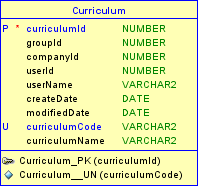
\includegraphics{curriculum.png}
	\caption{A mintatanterv relációséma}
\end{figure}

\subsection{Tantárgy}

Egy tantárgy mindig egy adott mintatantervhez kötődik. Három fontos attribútummal rendelkezik: tantárgykód, név és kredit érték.

\begin{figure}[H]
    \centering
	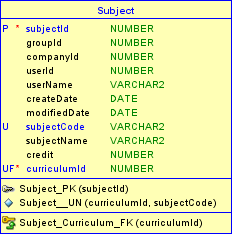
\includegraphics{subject.png}
	\caption{A tantárgy relációséma}
\end{figure}

\subsection{Kurzus Típus}

A kurzus típus egyed bevezetésére azért volt szükség, mert egy kurzusból többféle is létezhet és nem akartuk, hogy a forráskódot kelljen módosítani újabb típusok bevezetése esetén. Egy ilyen egyed tipikusan elmélet, gyakorlat, labor vagy vizsgakurzus típusokat reprezentál.

\begin{figure}[H]
    \centering
	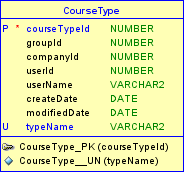
\includegraphics{course_type.png}
	\caption{A kurzus típus relációséma}
\end{figure}

\subsection{Kurzus}

Egy kurzus mindig egy tantárgyhoz és egy kurzus típushoz kötődik. A tantárgyhoz a kurzus adja meg a heti és féléves óraszámokat.

\begin{figure}[H]
    \centering
	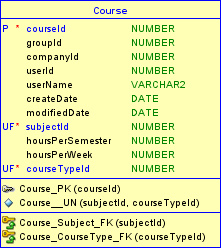
\includegraphics{course.png}
	\caption{A kurzus relációséma}
\end{figure}

\subsection{Félév}

A félév egyed, ahogyan azt a neve is sugallja egy egyetemi félévet reprezentál.

\begin{figure}[H]
    \centering
	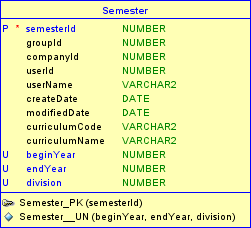
\includegraphics{semester.png}
	\caption{A félév relációséma}
\end{figure}

\subsection{Oktató}

Az oktató egyed bevezetésére azért volt szükség, mert nem biztos, hogy egy oktató azt a nevet szeretné megjeleníteni egy sillabuszban, mint amellyel a Liferay-es felhasználói fiókja is rendelkezik. Minden oktató egyedet össze lehet rendelni egy-egy valódi felhasználói fiókkal.

\begin{figure}[H]
    \centering
	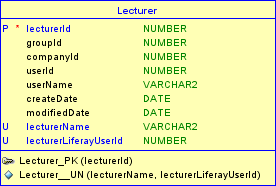
\includegraphics{lecturer.png}
	\caption{Az oktató relációséma}
\end{figure}

\subsection{Órarendi Kurzus}

Egy órarendi kurzus akkor jön létre, amikor egy adott félévben egy adott kurzust meghirdetnek a hallgatók számára.

\begin{figure}[H]
    \centering
	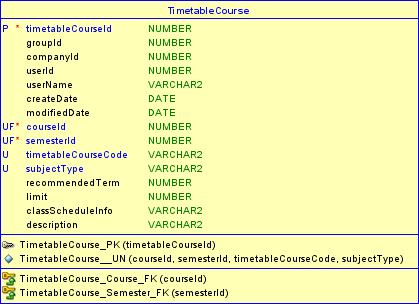
\includegraphics{timetable_course.png}
	\caption{Az órarendi kurzus relációséma}
\end{figure}

\subsection{Oktató - Órarendi Kurzus kapcsolat}

Ez az a tábla, amely képes eltárolni, hogy mely oktató, mely órarendi kurzushoz tartozik. Erre azért volt szükség, mert egy ilyen kurzusnak tetszőleges számú oktatója lehet és egy oktató is tetszőleges számú kurzust tarthat egyszerre egy félévben.

\begin{figure}[H]
    \centering
	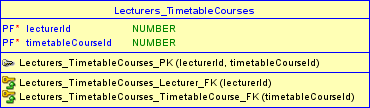
\includegraphics{lecturer_timetable_course.png}
	\caption{Az oktatókat és órarendi kurzusokat összekapcsoló relációséma}
\end{figure}

\subsection{Sillabusz}

Egy sillabusz mindig egy órarendi kurzushoz kötődik. Ez a tábla tartalmazza azon adatokat, amelyek félévente változhatnak egy újabb sillabusz kiadásakor.

\begin{figure}[H]
    \centering
	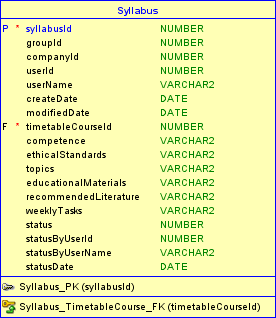
\includegraphics{syllabus.png}
	\caption{A sillabusz relációséma}
\end{figure}

\section{Szolgáltatások kialakítása}

A service.xml elkészítése után a \emph{gradlew buildService} parancs hatására lefut a Service Builder és minden szükséges interfészt és osztályt legenerál számunkra. A továbbiakban nincs más dolgunk, mint a szükséges szolgáltatások implementálása.

Liferay esetén kétféle szolgáltatást különböztetünk meg, helyi szolgáltatásokat és webszolgáltatásokat. Általában a webszolgáltatások csak egy interfészt nyújtanak a külvilág számára a helyi szolgáltatások elérésére, ezért én csak a helyi szolgáltatások létrehozását mutatom be.

Az egyes egyedekhez a \emph{hu.unideb.inf.service.impl} csomagban találhatóak meg azok az osztályok, melyeket újabb metódussal lehet bővíteni. Ebben a csomagban minden egyedhez két osztály tartozik: egy ServiceImpl és egy LocalServiceImpl nevekre végződő osztályok. Az előbbire a webszolgáltatások, az utóbbira pedig a helyi szolgáltatások miatt van szükség.

Az egyszerűség kedvéért az összes szolgáltatás közül csak a CurriculumLocalServiceImpl osztály lényeges részeit szeretném bemutatni.

\begin{minipage}{\linewidth}
\begin{lstlisting}[basicstyle=\small]
@ProviderType
public class CurriculumLocalServiceImpl
		extends CurriculumLocalServiceBaseImpl {
	
	public Curriculum getCurriculumByCode(
		String curriculumCode)
		throws SystemException,
			NoSuchCurriculumException {...}

	public Curriculum fetchCurriculumByCode(
		String curriculumCode)
		throws SystemException {...}

	public Curriculum addCurriculum(
		String curriculumCode, String curriculumName,
		ServiceContext serviceContext)
		throws PortalException, SystemException {...}

	public Curriculum updateCurriculum(
		long userId,
		long curriculumId,
		String curriculumCode,
		String curriculumName,
		ServiceContext serviceContext)
		throws PortalException, SystemException {...}

	public Curriculum deleteCurriculum(
		long curriculumId,
		ServiceContext serviceContext)
		throws PortalException, SystemException {...}
}
\end{lstlisting}
\end{minipage}

A getCurriculumByCode(...) metódus egy mintatanterv kódja alapján vissza tudja adni a megfelelő mintatantervet, viszont ha nincs a kódnak megfelelő adat az adatbázisban, akkor NoSuchCurriculumException kivételt fog dobni.

A fetchCurriculumByCode(...) metódus ugyan azt csinálja, mint a getCurriculumByCode(...), mindössze annyi a különbség a kettő között, hogy ez a metódus null értékkel tér vissza abban az esetben, ha az adatbázisban nem található meg a megfelelő mintatanterv.

Az addCurriculum(...) segítségével új mintatantervet lehet hozzáadni az adatbázishoz, az updateCurriculum(...) metódussal frissíteni lehet egy létező mintatanterv adatait, a deleteCurriculum(...) meghívásával pedig törölni lehet egy mintatantervet az adatbázisból. Ha törlés során kiderülne, hogy a törlendő mintatantervhez legalább egy tantárgy is kapcsolódik, akkor DeleteSubjectsFirstException kivétel váltódik ki és a törlés nem hajtódik végre. Az add és update metódusok validációt is végrehajtanak. Abban az esetben, ha a létrehozandó vagy módosítandó egyed egyik attribútuma nem megfelelő értékkel rendelkezik, akkor szintén kivétel dobódik és a művelet végrehajtása megszakad, amely hatására hibaüzenetet lehet megjeleníteni a felhasználói felületen.

A webszolgáltatások miatt jelen lévő CurriculumServiceImpl osztályon belül, szinte minden metódus először azt ellenőrzi, hogy a felhasználó rendelkezik-e a megfelelő jogosultsággal a művelet végrehajtására. Ha igen, akkor a CurriculumLocalServiceImpl osztályon belül található megfelelő metódus hívódik meg, ha viszont valamilyen oknál fogva a felhasználó nem rendelkezne a megfelelő jogosultsággal, akkor PrincipalException váltódik ki és biztonsági okokból a művelet végrehajtása el sem kezdődik.

A szolgáltatások implementálása után újra kell generáltatni a Service Builder által létrehozott többi forráskódot.

\section{Portlet létrehozása}

A szolgáltatások kialakítása utána már csak egy felhasználói interfész létrehozására volt szükség. Követelményként az volt meghatározva, hogy legyen egy adminisztrációs felület, ahol a tantárgyak alapadatait meg lehet adni. A sillabusz kezelő alkalmazás adminisztráció felületét ott helyeztem el, ahol a többi alkalmazás adminisztrációs felülete is megtalálható, azaz az Liferay 7.0-ban a régi vezérlőpultot felváltó oldalsáv "Tartalom" menüpontja alatt.

A felület létrehozására mindössze egy portlet létrehozására, a megfelelő műveletek definiálására és a megjelenítő oldalak kialakítására volt szükség. A technikai részletekbe nem szeretnék belemenni, mert egy teljes diplomamunka is kevés lenne mindezek elmagyarázására.

\section{Jogosultságkezelés}

A kialakított felületen minden elem esetén ellenőrizve van, hogy a felhasználó rendelkezik-e a megfelelő jogosultságokkal, annak használatára. Ha nem rendelkezik, akkor az elem vagy akár az egész oldal egyszerűen nem jelenik meg, még hibaüzenet sem jelenik meg arról, hogy nincs meg a felhasználónak a megfelelő joga, mert ezzel csak a biztonságosság szintjét csökkentettem volna.

A Liferay a szerepkör alapú jogosultságkezelést támogatja. A portál három különböző típusú szerepkört különít el, a \emph{normál}, a \emph{webhely} és a \emph{szervezet} típusú szerepköröket. A jogosultságkezelés beállításához mindössze egy megfelelő típusú szerepkört kell létrehozni és magára a szerepkörre kell meghatározni, hogy mely jogosultságokkal rendelkezik. Ezután a szerepkört hozzá lehet rendelni egy felhasználóhoz és máris rendelkezik a szükséges jogosultságokkal. Sok helyen az ilyen fajta jogosultságkezelésre "Role Object Pattern" névként szokás hivatkozni, amely egy széles körben elfogadott tervezési mintának felel meg.

Forráskód szinten a jogosultságkezelés kialakításához a következő dolgokra volt szükségem:
\begin{enumerate}
\item jogosultságok definiálása,
\item jogosultság ellenőrző osztályok kialakítása,
\item jogosultság ellenőrzés a szükséges helyeken.
\end{enumerate}

\subsection{Jogosultságok definiálása}

A sillabusz kezelő alkalmazás esetén minden jogosultságot a syllabus-manager-service projekten belül az \emph{src/main/resources/META-INF/resource-actions/default.xml} állományban definiáltam. A Liferay két szintű jogosultságokat különböztet meg: felsőbb szintű (top level) és erőforrás szintű jogosultságokat. Felsőbb szintű akkor lesz egy jogosultság, ha nem tartozik semmilyen erőforráshoz, például egyedhez. Előfordulhat, hogy egyes helyeken a felsőbb szintű jogosultságokat a magyar szakirodalomban általános jogosultságoknak neveznek.

\begin{table}[H]
	\caption{Példák felsőbb szintű jogosultságokra}
	\centering
	\begin{tabular}{| l | l | l |}
	\hline
	\textbf{Jogosultság neve} & \textbf{Leírás} \\
	\hline
	ADD\_CURRICULUM & Mintatanterv hozzáadási jog \\
	\hline
	DELETE\_CURRICULUMS & Csoportos mintatanterv törlési jog \\
	\hline
\end{tabular}
\end{table}

\begin{table}[H]
	\caption{Példák mintatanterv esetén erőforrás szintű jogosultságokra}
	\centering
	\begin{tabular}{| l | l | l |}
	\hline
	\textbf{Jogosultság neve} & \textbf{Leírás} \\
	\hline
	DELETE & Egyéni törlési jog egy adott mintatantervre \\
	\hline
	VIEW & Megtekintési jog egy adott mintatantervre \\
	\hline
\end{tabular}
\end{table}

\subsection{Jogosultság ellenőrző osztályok kialakítása}

Ezeket az osztályokat a kódismétlés csökkentése érdekében kellett kialakítanom. Mindegyik tartalmaz egy \emph{check} és \emph{contains} nevű metódust. A check metódus PrincipalException kivételt dob minden olyan esetben, amikor a felhasználó nem rendelkezik az ellenőrzött jogosultsággal, a contains pedig igaz/hamis értékkel tér vissza annak függvényében, hogy a felhasználó rendelkezik-e a megfelelő jogosultságokkal.

Ezek a jogosultságokat ellenőrző osztályok a \emph{hu.unideb.inf.service.permission} csomagon belül lettek elhelyezve. Felsőbb szintű jogosultságok ellenőrzésére a ModelPermission osztályt, az erőforrás szintűekre pedig az egyes egyedeknek külön létrehozott osztályokat lehet használni.

\subsection{Jogosultság ellenőrzés a szükséges helyeken}

A jogosultság ellenőrzése úgy történik, hogy a szükséges helyen a megfelelő jogosultság ellenőrző osztály megfelelő metódusa a megfelelő paraméterekkel hívódik meg. Jó példa erre a sillabuszok listázásánál végzett erőforrás szintű ellenőrzés:

\begin{minipage}{\linewidth}
\begin{lstlisting}[basicstyle=\small]
<c:if test='<%=SyllabusPermission.contains(
	permissionChecker, syllabus.getSyllabusId(), "VIEW")%>'>
	...
</c:if>
\end{lstlisting}
\end{minipage}

\noindent A példában szereplő kód azt ellenőrzi, hogy a felhasználó fel van-e jogosítva az adott sillabusz megtekintésére vagy sem.

\section{Munkafolyamat támogatás}

Az egyik legfontosabb követelmény a munkafolyamat támogatása volt. Ezt a portálba épített keretrendszer segítségével tettem lehetővé. A munkafolyamat kialakítása viszonylag egyszerű folyamat:
\begin{enumerate}
\item Asset integráció.
\item Új attribútumok felvétele.
\item Szolgáltatások módosítása.
\item WorkflowHandler osztály létrehozása.
\end{enumerate}

\subsection{Asset integráció}

Asset integráció alatt azt kell érteni, hogy egy entitás kezelhetővé válik az Asset Publisher nevű portleten keresztül. Erre a részre amúgy is szükség lett volna, mert követelményként volt meghatározva, hogy egy sillabuszt az Asset Publisher-en keresztül kell tudni létrehozni, módosítani és legfőképpen megjeleníteni.

\subsection{Új attribútumok felvétele}

A sillabusz egyed esetén négy új attribútum felvételére volt szükség:
\begin{table}[H]
	\centering
	\begin{tabular}{| l | l | l |}
	\hline
	\textbf{Attribútum neve} & \textbf{Leírás} \\
	\hline
	status & Az egyed munkafolyamatbeli állapotát jelzi \\
	\hline
	statusByUserId & Az egyedet létrehozó felhasználó azonosítója \\
	\hline
	statusByUserName & Az egyedet létrehozó felhasználóneve \\
	\hline
	statusDate & Az egyed munkafolyamatbeli állapotának utolsó módosítási dátuma \\
	\hline
\end{tabular}
\end{table}

\subsection{Szolgáltatások módosítása}

A SyllabusLocalServiceImpl osztályon belül található metódusokat úgy kellett módosítani, hogy hozzáadáskor és frissítéskor új munkafolyamat induljon el, törléskor pedig szűnjön meg az összes kapcsolódó munkafolyamat.

Ugyan ebben az osztályban szükség volt még egy újabb, updateStatus(...) nevű metódus bevezetésére is. A metódus megfelelő paraméterekkel történő meghívásával lehet állítani az egyes sillabuszok munkafolyamatbeli állapotait.

\subsection{WorkflowHandler komponens létrehozása}

A Liferay a 7.0 verzió megjelenése óta komponensekkel és modulokkal dolgozik. Mindezt az OSGI keretrendszer bevezetése tette lehetővé. Munkafolyamat kezelésnél nekem is egy újabb komponenst kellett létrehoznom, annak érdekében, hogy az OSGI futtatórendszer tudomást szerezzen arról, hogy a sillabusz egyedek is támogatják a portálba épített munkafolyamat keretrendszert.

\chapter{Az alkalmazás bemutatása}

Számtalan képet lehetne itt elhelyezni arról, hogy hogyan is néz ki a valóságban a sillabusz kezelő alkalmazás, de az oldalakkal való takarékosság érdekében csak a leglényegesebb funkciókat szeretném bemutatni felhasználói szemszögből.

\section{Főoldal}

A főoldal egész egyszerű felépítést kapott. Ezen az oldalon mindössze egy menüsor és egy breadcrumb található meg. A képen jól látszik a bal oldali oldalsáv és a benne elhelyezett \emph{Sillabusz Adminisztráció} menüpont, amely a korábbi Liferay verziókban megtalálható vezérlőpultot váltotta fel. A menüsor és breadcrumb szinte az összes oldalon ugyan így néz ki, értelemszerűen az utóbbi elem egyes helyeken több bejegyzést is tartalmaz, nem csak egyet, mint ahogyan az a főoldalon is látható.

A menüsor \emph{Megtekintés} menüpontja alatt négy elem található: \emph{Mintatantervek}, \emph{Kurzus típusok}, \emph{Félévek} és \emph{Oktatók}.

Az \emph{Új} menüpont alatt minden egyed felsorolásra került. A megfelelő egyed kiválasztása után a rendszer lehetőséget biztosít egy új elem hozzáadására.

A \emph{Veszélyzóna} menüpont olyan műveleteket foglal magában, amelyek az egész rendszer működését befolyásolhatják. Jelenleg két almenüpont tartozik hozzá: \emph{Adatbázis törlése} és \emph{Exportálás / Importálás}.

A menüsor utolsó eleme egy halványszürke, áthúzott betűkkel megjelenített \emph{Importálás} menüpont. Ez azért így jelenik meg, mert használata erősen ellenjavallott, erre csak az eredetileg az egyetemtől kapott adatok betöltése során volt szükségem.

\begin{figure}[H]
    \centering
	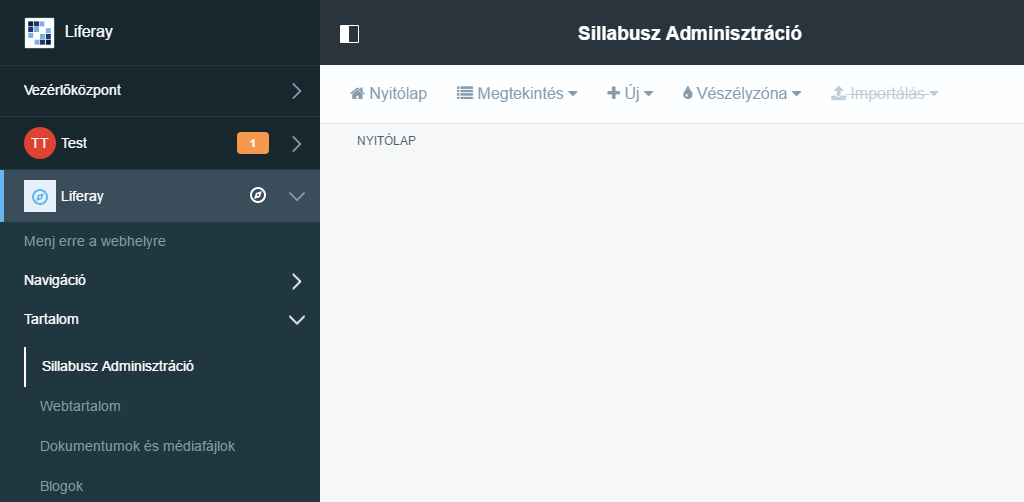
\includegraphics[width=\textwidth]{sm_main_page.png}
	\caption{A sillabusz kezelő portlet főoldala}
\end{figure}

\section{Listázó oldalak}

Minden általam definiált egyedhez külön-külön listázó oldalt hoztam létre. A kialakítás során törekedtem egyfajta hierarchikus megjelenítésre, ezt úgy értem el, hogy a mintatanterveket, illetve a féléveket listázó oldalakból kiindulva el lehet jutni a sillabuszok megjelenítéséig.

Minden listázó oldalon minden egyes bejegyzés mellett található egy \emph{Műveletek} menüpont. Ez egyetlen egy esetet kivéve minden egyed esetén három elemet tartalmaz: \emph{Szerkesztés}, \emph{Jogosultságok} és \emph{Törlés}. Az egyetlen kivétel ez alól az órarendi kurzusok, ahol megtalálható egy negyedik elem is, a \emph{Megtekintés} menüpont. Ezt a menüpontot kiválasztva lehet eljutni az adott órarendi kurzushoz tartozó sillabuszokat listázó oldalra.

\begin{figure}[H]
    \centering
	
\includegraphics{sm_list_actions_timetable_course.png}
	\caption{Egy listázóban található elem lehetséges műveletei}
\end{figure}

\begin{figure}[H]
    \centering
	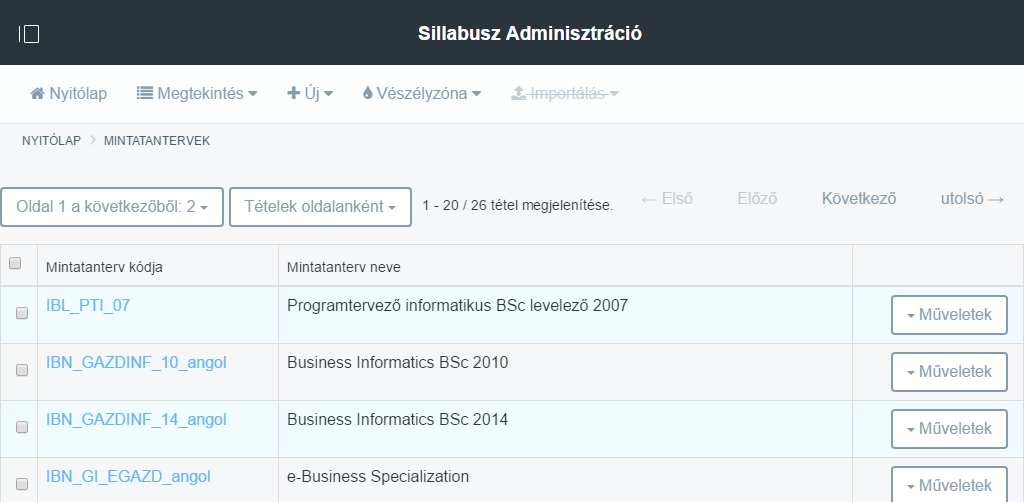
\includegraphics[width=\textwidth]{sm_curriculum_list.png}
	\caption{A mintatanterv listázó}
\end{figure}

\begin{figure}[H]
    \centering
	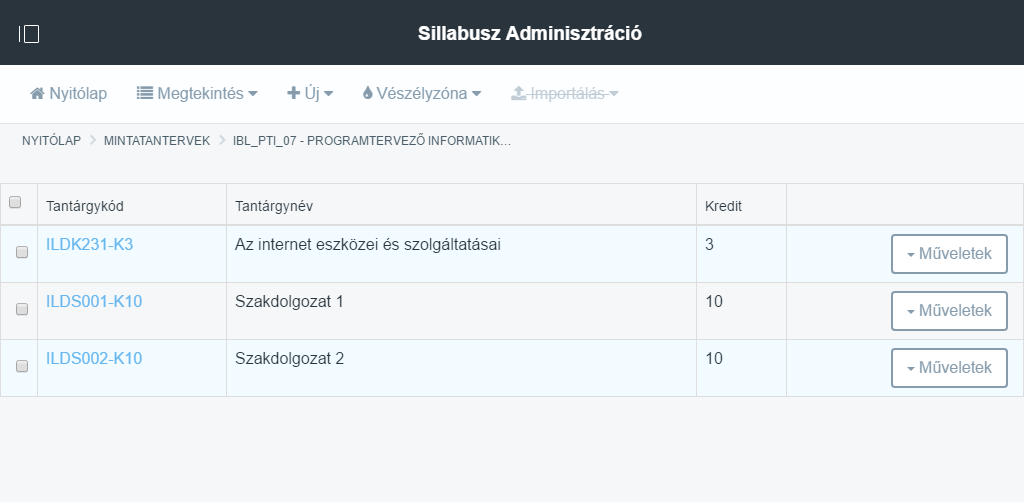
\includegraphics[width=\textwidth]{sm_subject_list.png}
	\caption{A tantárgy listázó}
\end{figure}

\begin{figure}[H]
    \centering
	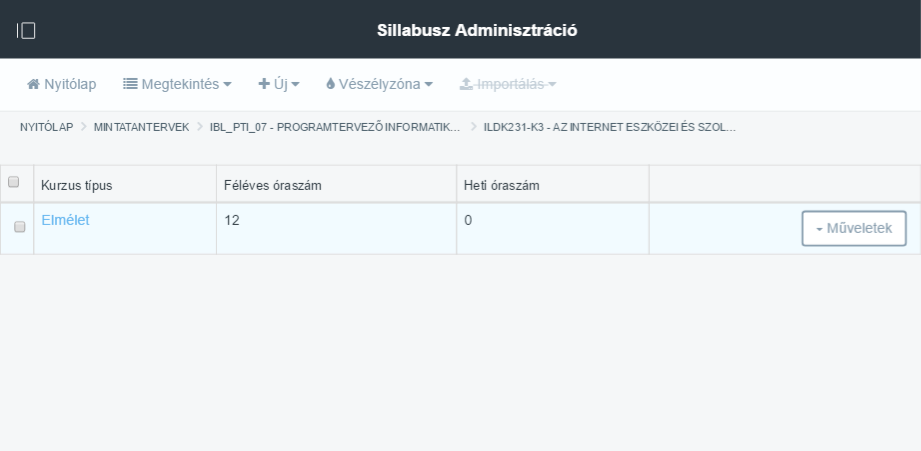
\includegraphics[width=\textwidth]{sm_course_list.png}
	\caption{A kurzus listázó}
\end{figure}

\begin{figure}[H]
    \centering
	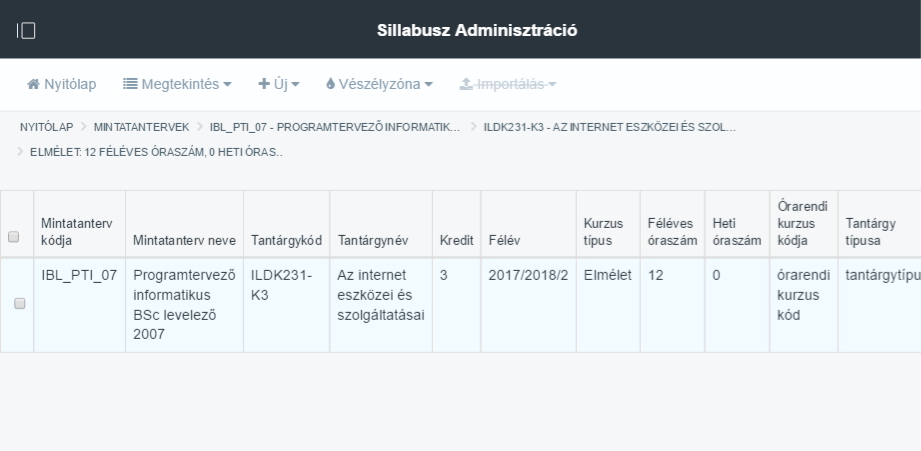
\includegraphics[width=\textwidth]{sm_timetable_course_list.png}
	\caption{Az órarendi kurzus listázó}
\end{figure}

\begin{figure}[H]
    \centering
	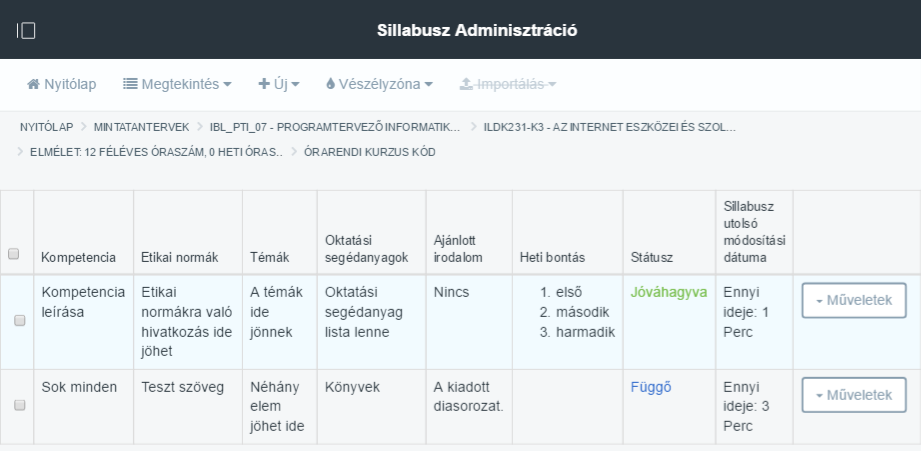
\includegraphics[width=\textwidth]{sm_syllabus_list.png}
	\caption{A sillabusz listázó}
\end{figure}

\section{Sillabusz létrehozása}

Egy sillabusz hozzáadása során az első lépés mindig az alapinformációk megadása. Az adatok megadása alatt a megfelelő egyedek kiválasztását kell érteni. Az oldalon elhelyezett legördülő menük tartalma az eggyel felette lévő menü értékétől függ, kivéve a legelső esetben. Ezt a fajta működést egy példával szemléltetve könnyebb megérteni: csak azon tantárgyak kerülnek kilistázásra, amelyek a kiválasztott mintatantervhez tartoznak, azaz a tantárgylistázó tartalma függ a kiválasztott mintatantervtől.

Az alapinformációk meghatározása után szöveges beviteli mezők találhatóak. Ezek mindegyike kötelező mező, azaz, ha egyiket valaki nem töltené ki, akkor hibaüzenetet küld a rendszer arról, hogy a mező tartalma üres. A legutolsó szöveges beviteli mező egy WYSIWYG szerkesztő.

\begin{figure}[H]
    \centering
	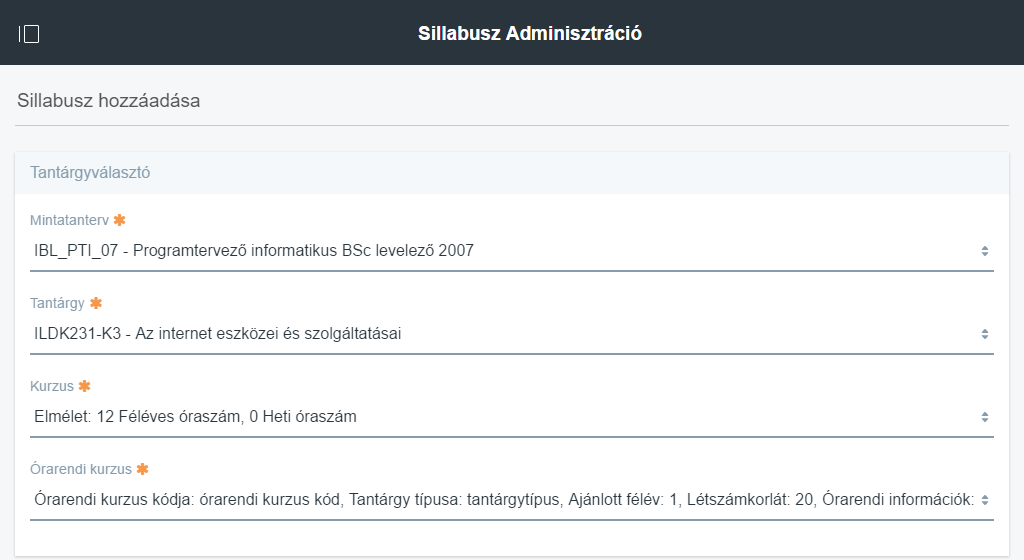
\includegraphics[width=\textwidth]{sm_syllabus_add_1.png}
	\caption{Egy sillabusz létrehozása 1/4}
\end{figure}

\begin{figure}[H]
    \centering
	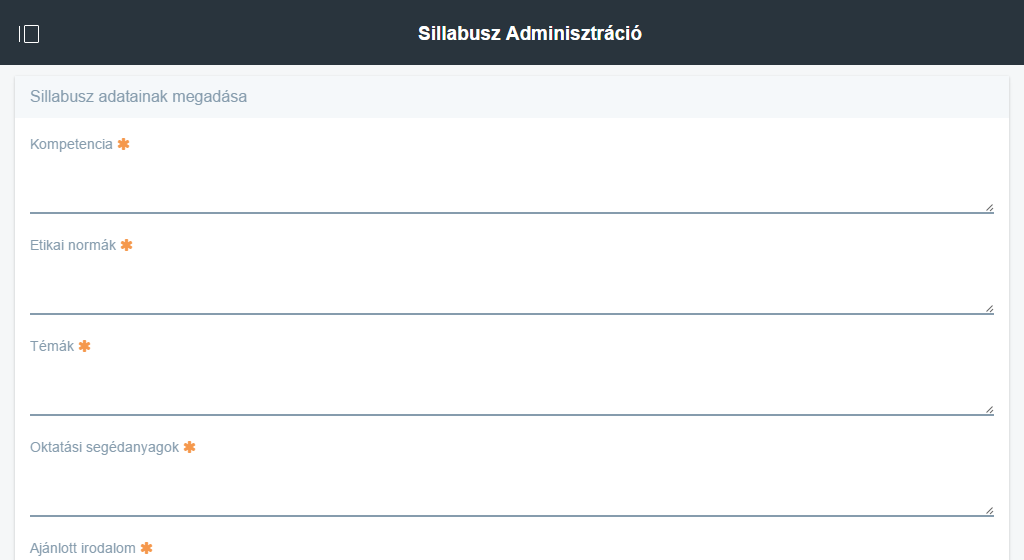
\includegraphics[width=\textwidth]{sm_syllabus_add_2.png}
	\caption{Egy sillabusz létrehozása 2/4}
\end{figure}

\begin{figure}[H]
    \centering
	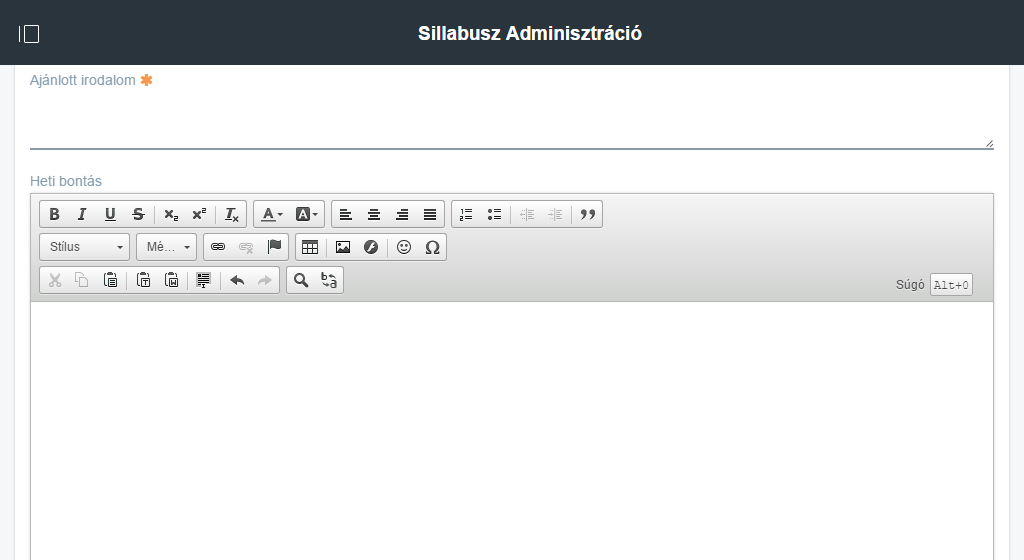
\includegraphics[width=\textwidth]{sm_syllabus_add_3.png}
	\caption{Egy sillabusz létrehozása 3/4}
\end{figure}

A szöveges beviteli mezők után megtalálható még egy utolsó rész is, amely a Liferay Asset Publisher miatt jelenik meg. Itt lehet címkéket és kapcsolódó tartalmakat hozzárendelni a létrehozandó sillabuszhoz. Az Asset Publisher számos beállítási lehetőséggel rendelkezik, a címkék alapján történő szűrés az egyik leggyakrabban használt funkciója.

\begin{figure}[H]
    \centering
	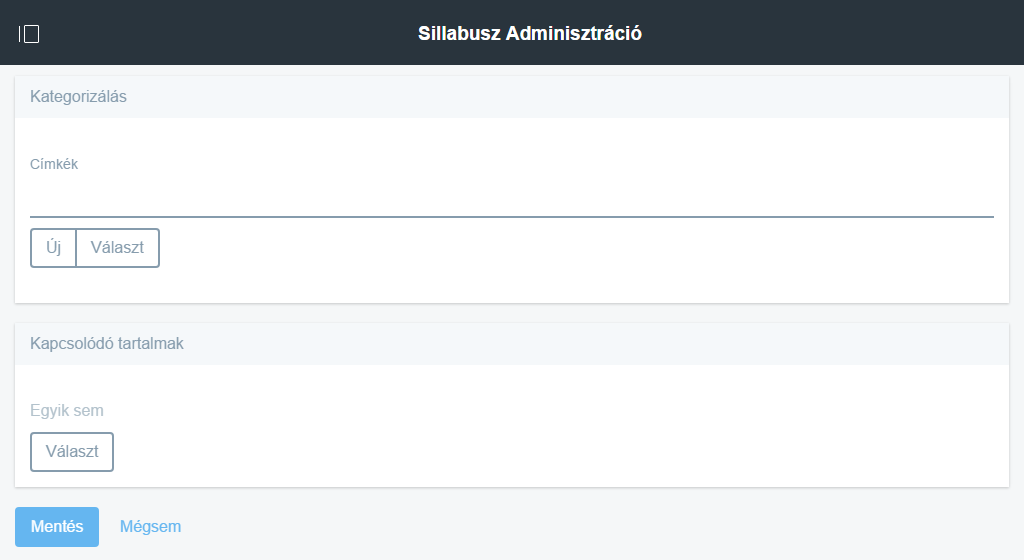
\includegraphics[width=\textwidth]{sm_syllabus_add_4.png}
	\caption{Egy sillabusz létrehozása 4/4}
\end{figure}

\section{Importálás / Exportálás}

Az alkalmazás képes az összes általa tárolt adat exportálására és ezen exportált adatok újbóli importálására is. Jelenleg a rendszer támogatja mind az XML, mind a CSV formátumú állományok kezelését. A sillabuszok exportálása gombok használata esetén, nem csak a sillabuszok, hanem az összes mintatanterv, tantárgy, kurzus és órarendi kurzus is kiexportálódik, ezért nincs külön gomb ezekre az egyedekre elhelyezve az oldalon.

\begin{figure}[H]
    \centering
	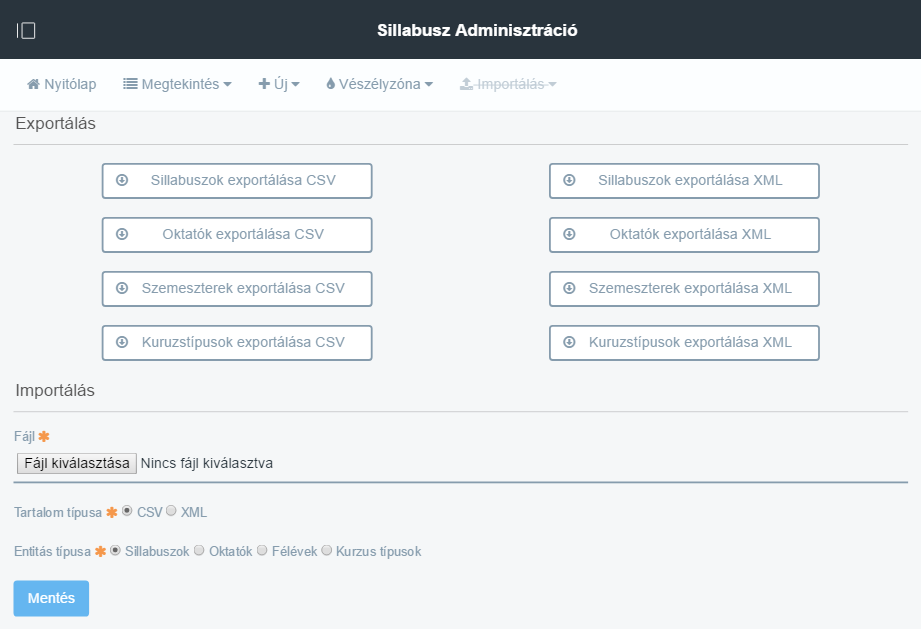
\includegraphics[width=\textwidth]{sm_import_export.png}
	\caption{Az importálás/exportálás oldala}
\end{figure}

\chapter{Összefoglalás}

Büszkén jelenthetem ki, hogy az elkészült sillabusz kezelő alkalmazás egyetlen egy esettől eltekintve teljes egészében megfelel a vele szemben támasztott követelményeknek. Az alkalmazás fejlesztése során sikerült elérnem egy olyan szoros integrációt magával a Liferay tartalomkezelő rendszerrel, hogy az alkalmazás telepítése után szinte senki sem tudná megmondani, hogy az alkalmazás nem beépített portlet volna. Az egyetlen egy nem megvalósított követelmény a sillabusz duplikálása volt, ugyanis a program fejlesztése közben kiderült, hogy a kari honlap a továbbiakban garantáltan nem Liferay alapokra fog épülni, ezért végül nem láttam értelmét ezen funkció beépítésének.

Az alkalmazás fejlesztése közben jelentős új tudásra tettem szert. Egyrészt megtanultam egy mindenki által elismert, már több mint tizenhét éve a piacon lévő és széles körben használt tartalomkezelő rendszer használatát és a rendszerre történő fejlesztés különböző módszereit, másrészt pedig olyan problémákkal találtam szemben magamat az elmúlt két évben, amelyekkel éles körülmények között is találkoznak a szoftverfejlesztők. A legnagyobb probléma, amelyet le kellett küzdenem a verziómigráció volt. Mire megtanultam a Liferay 6.2-re való fejlesztés folyamatát és otthon éreztem magam benne, addigra megjelent a 7.0 verzió a rengeteg újításával együtt, ezért egy csomó mindent újra kellett írnom ezen alapvető változtatások miatt. Ennek a migrációnak köszönhetően megtanultam használni a Gradle, a Blade CLI eszközöket, elsajátítottam az Apache Velocity és Apache FreeMarker templating motorok \cite{apache-velocity} használatát, jobban megértettem, hogy miért van szükség egy szolgáltatásokat nyújtó interfész kialakítására egy ilyen vagy ehhez hasonló alkalmazások esetén, otthonosabban érzem magam JavaScript kódok írása közben, jobban rálátok a biztonsági kérdésekre, illetve elsajátítottam az Alloy UI keretrendszer \cite{alloyui} használatának alapjait.

Természetesen, mint minden alkalmazás ez sem teljes. Mindig mindent tovább lehet fejleszteni, ez igaz a sillabusz kezelő alkalmazásra is. Talán az egyik lehetséges továbbfejlesztési lehetőség az Application Display Template-ek (ADT) támogatása lenne, amely lehetővé tenné, hogy az Asset Publisher-en keresztül megjelenített sillabuszok kinézetének futás időben történő megváltoztatását. Az ADT támogatja mind az Apache Velocity, mind az Apache FreeMarker templating \cite{apache-velocity, apache-freemarker} motorokat, így mindenki tetszés szerint azt használhatja megjelenítő sablonok készítésére, amelyik szimpatikusabb számára.

Egy másik továbbfejlesztési lehetőség a portálba épített keresőmotor integrációja lehet. Ahhoz, hogy a tartalmak között keresni lehessen, az adatbázisban lévő adatok megfelelő módon történő indexelésére van szükség, amelyre a Liferay szintén egy saját fejlesztésű keretrendszert biztosít a fejlesztők számára.

Harmadik továbbfejlesztési lehetőségként az általam kialakított webszolgáltatások esetén a jogosultságkezelés átalakítását tudom javasolni. Jelenleg van olyan része a szolgáltatásoknak, amelyek akkor is meghívhatóak, amikor a szolgáltatást megszólító felhasználó nincs feljogosítva a szolgáltatás használatára. A szolgáltatások esetén az egyedek hozzáadása, frissítése és törlése minden esetben le van védve az illetéktelen hozzáférés ellen, viszont az adatok lekérdezésére szolgáltató interfészek során csak egy részük esetén lett jogosultságkezelés kialakítva. Amikor még ezeket a szolgáltatások alakítottam ki, még úgy gondoltam, hogy ilyen tantárgyi adatok lekérdezéséből nem lehet baj, de mivel a felhasználói felület esetén minden esetben megtörténik az összes jogosultság ellenőrzése, ezért ma már jobbnak látom, ha a szolgáltatások esetén is mindenhol ellenőrzésre kerülnének ezen hozzáférési jogok.

\clearpage
\addcontentsline{toc}{chapter}{Köszönetnyilvánítás}
\chapter*{Köszönetnyilvánítás}

Ez a diplomamunka nem jöhetett volna létre a családom, a barátaim, az egyetem, a témavezetőm, illetve a Liferay Hungary Kft. támogatása nélkül, ezért szeretném megragadni az alkalmat arra, hogy mindenkinek köszönetet mondjak, aki az elmúlt években mellettem állt és lehetőséget teremtett arra, hogy ez a diplomamunka elkészülhessen.

Köszönöm a családomnak, amiért az elmúlt két évben mindent megtettek azért, hogy idáig eljuthassak az életben, illetve mindazért, amiért mindvégig kitartottak mellettem.

Köszönöm a barátaimnak is a sok támogatást, közülük legfőképpen László Zsolt segítségét, aki néhány évvel ezelőtt bevezetett a \LaTeX szövegformázó rendszer használatába és rendelkezésemre bocsátotta egy általa készített korábbi dokumentum vázlatát.

Végül szeretném megköszönni témavezetőmnek, Dr. Adamkó Attilának, amiért lehetőséget teremtett arra, hogy díjmentesen részt vehessek a Liferay Hungary Kft. által tartott \emph{Developing for the Liferay Platform 1} című képzésen, illetve köszönet illeti mindazért a maradék támogatásáért is, amit az elmúlt néhány évben nyújtott számomra.

% Ábrajegyzék (nem kell, helyette van függelék!)
% \listoffigures

% Irodalomjegyzék
% Tartalomjegyzékhez így lehet hozzáadni: http://latex-community.org/forum/viewtopic.php?t=9446
\clearpage
\addcontentsline{toc}{chapter}{Irodalomjegyzék}
\begin{thebibliography}{10}

\section*{Könyvek}

\bibitem{liferay-in-action} Richard Sezov Jr.: Liferay in Action, 2011, ISBN 9781935182825
\bibitem{java-se-platformon} Kövesdán Gábor: Szoftverfejlesztés Java SE platformon, 2014, ISBN 9789639863354
\bibitem{java-ee-platformon} Balogh Péter, Berényi Zsolt, Dévai István, Imre Gábor, Soós István, Tóthfalussy Balázs: Szoftverfejlesztés Java EE platformon, 2007, ISBN 9789639131972
\bibitem{szoftverrendszerek-fejlesztese} Ian Sommerville: Szoftverrendszerek fejlesztése, 2007, ISBN 9789635454785
\bibitem{packt-restful} Jose Sandoval: RESTful Java Web Services, 2009, ISBN 9781847196460

\section*{Online források}

\bibitem{liferay} Liferay \\ \small\url{https://www.liferay.com/}
\bibitem{jsr286} JSR 286 - Portlet Specification 2.0 \\ \small\url{https://www.jcp.org/en/jsr/detail?id=286}
\bibitem{sillabusz} Sillabusz \\ \small\url{https://hu.wiktionary.org/wiki/sillabusz}
\bibitem{liferay-dev-1} Developing for the Liferay Platform 1 \\ \small\url{https://www.liferay.com/services/training/6.2/topics/developer-1}
\bibitem{redmine} Redmine \\ \small\url{http://www.redmine.org/}
\bibitem{statcounter} StatCounter \\ \small\url{http://gs.statcounter.com/os-market-share}
\bibitem{gradle} Gradle \\ \small\url{https://gradle.org/}
\bibitem{blade-cli} Blade CLI \\ \small\url{https://dev.liferay.com/develop/tutorials/-/knowledge_base/7-0/blade-cli}
\bibitem{apache-ant} Apache Ant \\ \small\url{http://ant.apache.org/}
\bibitem{apache-maven} Apache Maven \\ \small\url{https://maven.apache.org/}
\bibitem{apache-velocity} Apache Velocity \\ \small\url{http://velocity.apache.org/}
\bibitem{apache-freemarker} Apache FreeMarker \\ \small\url{http://freemarker.org/}
\bibitem{jquery} jQuery \\ \small\url{https://jquery.com/}
\bibitem{alloyui} Alloy UI \\ \small\url{http://alloyui.com/}
\bibitem{google-seo-book} Google Keresőmotor-optimalizálási
útmutató kezdőknek \\ \small\url{https://static.googleusercontent.com/media/www.google.hu/en/hu/intl/hu/webmasters/docs/search-engine-optimization-starter-guide-hu.pdf}

\end{thebibliography}

%\appendix
%\chapter{Első függelék}

%\section{leírás}

%Ide kerülnek azok a nagyobb méretű táblázatok, ábrák.
%Ide helyezhető el továbbá a kérdőíves felmérés alapjául szolgáló dokumentumok, továbbá a statisztikai és matematikai számítások alaptáblái is.
%Egyes esetekben rövidebb szöveges dokumentumok (pl. szerződése, jogszabály részletek, stb.) is helyet kaphatnak itt.

%\chapter{Második függelék}

%függelékes cucc

\end{document}

% \vspace{10mm}

% \noindent A korrigált, empirikus szórás képlete:

%\begin{equation}
% s_e^{*} = \sqrt{\frac{\mathlarger{\sum}\limits_{i = 1}^{n} \left( x_i - \bar{x} \right)^2 }{n - 1}}
% \end{equation}

% \vspace{10mm}

% Irodalom idézése

% \noindent Az \cite{studalccons} forrásban leírtak szerint...

% Félkövér betűstílus
% \textbf{Az alkalmazott operátorok a következők voltak:}

% Dőlt betűstílus
% \textit{Amik ezt csinálták}

% Hasonló
% \emph{De ez lehet, hogy szebb formázás}

% Színezés
% {\color{red}Színezni is tudsz}

% Nem kell beljebb kezdeni
% \noindent Ha nem akarod, hogy beljebb kezdje

% \label{results}